% Options for packages loaded elsewhere
% Options for packages loaded elsewhere
\PassOptionsToPackage{unicode}{hyperref}
\PassOptionsToPackage{hyphens}{url}
%
\documentclass[
  spanish,
  letterpaper,
]{book}
\usepackage{xcolor}
\usepackage[margin=1in]{geometry}
\usepackage{amsmath,amssymb}
\setcounter{secnumdepth}{5}
\usepackage{iftex}
\ifPDFTeX
  \usepackage[T1]{fontenc}
  \usepackage[utf8]{inputenc}
  \usepackage{textcomp} % provide euro and other symbols
\else % if luatex or xetex
  \usepackage{unicode-math} % this also loads fontspec
  \defaultfontfeatures{Scale=MatchLowercase}
  \defaultfontfeatures[\rmfamily]{Ligatures=TeX,Scale=1}
\fi
\usepackage{lmodern}
\ifPDFTeX\else
  % xetex/luatex font selection
\fi
% Use upquote if available, for straight quotes in verbatim environments
\IfFileExists{upquote.sty}{\usepackage{upquote}}{}
\IfFileExists{microtype.sty}{% use microtype if available
  \usepackage[]{microtype}
  \UseMicrotypeSet[protrusion]{basicmath} % disable protrusion for tt fonts
}{}
\makeatletter
\@ifundefined{KOMAClassName}{% if non-KOMA class
  \IfFileExists{parskip.sty}{%
    \usepackage{parskip}
  }{% else
    \setlength{\parindent}{0pt}
    \setlength{\parskip}{6pt plus 2pt minus 1pt}}
}{% if KOMA class
  \KOMAoptions{parskip=half}}
\makeatother
% Make \paragraph and \subparagraph free-standing
\makeatletter
\ifx\paragraph\undefined\else
  \let\oldparagraph\paragraph
  \renewcommand{\paragraph}{
    \@ifstar
      \xxxParagraphStar
      \xxxParagraphNoStar
  }
  \newcommand{\xxxParagraphStar}[1]{\oldparagraph*{#1}\mbox{}}
  \newcommand{\xxxParagraphNoStar}[1]{\oldparagraph{#1}\mbox{}}
\fi
\ifx\subparagraph\undefined\else
  \let\oldsubparagraph\subparagraph
  \renewcommand{\subparagraph}{
    \@ifstar
      \xxxSubParagraphStar
      \xxxSubParagraphNoStar
  }
  \newcommand{\xxxSubParagraphStar}[1]{\oldsubparagraph*{#1}\mbox{}}
  \newcommand{\xxxSubParagraphNoStar}[1]{\oldsubparagraph{#1}\mbox{}}
\fi
\makeatother

\usepackage{color}
\usepackage{fancyvrb}
\newcommand{\VerbBar}{|}
\newcommand{\VERB}{\Verb[commandchars=\\\{\}]}
\DefineVerbatimEnvironment{Highlighting}{Verbatim}{commandchars=\\\{\}}
% Add ',fontsize=\small' for more characters per line
\usepackage{framed}
\definecolor{shadecolor}{RGB}{241,243,245}
\newenvironment{Shaded}{\begin{snugshade}}{\end{snugshade}}
\newcommand{\AlertTok}[1]{\textcolor[rgb]{0.68,0.00,0.00}{#1}}
\newcommand{\AnnotationTok}[1]{\textcolor[rgb]{0.37,0.37,0.37}{#1}}
\newcommand{\AttributeTok}[1]{\textcolor[rgb]{0.40,0.45,0.13}{#1}}
\newcommand{\BaseNTok}[1]{\textcolor[rgb]{0.68,0.00,0.00}{#1}}
\newcommand{\BuiltInTok}[1]{\textcolor[rgb]{0.00,0.23,0.31}{#1}}
\newcommand{\CharTok}[1]{\textcolor[rgb]{0.13,0.47,0.30}{#1}}
\newcommand{\CommentTok}[1]{\textcolor[rgb]{0.37,0.37,0.37}{#1}}
\newcommand{\CommentVarTok}[1]{\textcolor[rgb]{0.37,0.37,0.37}{\textit{#1}}}
\newcommand{\ConstantTok}[1]{\textcolor[rgb]{0.56,0.35,0.01}{#1}}
\newcommand{\ControlFlowTok}[1]{\textcolor[rgb]{0.00,0.23,0.31}{\textbf{#1}}}
\newcommand{\DataTypeTok}[1]{\textcolor[rgb]{0.68,0.00,0.00}{#1}}
\newcommand{\DecValTok}[1]{\textcolor[rgb]{0.68,0.00,0.00}{#1}}
\newcommand{\DocumentationTok}[1]{\textcolor[rgb]{0.37,0.37,0.37}{\textit{#1}}}
\newcommand{\ErrorTok}[1]{\textcolor[rgb]{0.68,0.00,0.00}{#1}}
\newcommand{\ExtensionTok}[1]{\textcolor[rgb]{0.00,0.23,0.31}{#1}}
\newcommand{\FloatTok}[1]{\textcolor[rgb]{0.68,0.00,0.00}{#1}}
\newcommand{\FunctionTok}[1]{\textcolor[rgb]{0.28,0.35,0.67}{#1}}
\newcommand{\ImportTok}[1]{\textcolor[rgb]{0.00,0.46,0.62}{#1}}
\newcommand{\InformationTok}[1]{\textcolor[rgb]{0.37,0.37,0.37}{#1}}
\newcommand{\KeywordTok}[1]{\textcolor[rgb]{0.00,0.23,0.31}{\textbf{#1}}}
\newcommand{\NormalTok}[1]{\textcolor[rgb]{0.00,0.23,0.31}{#1}}
\newcommand{\OperatorTok}[1]{\textcolor[rgb]{0.37,0.37,0.37}{#1}}
\newcommand{\OtherTok}[1]{\textcolor[rgb]{0.00,0.23,0.31}{#1}}
\newcommand{\PreprocessorTok}[1]{\textcolor[rgb]{0.68,0.00,0.00}{#1}}
\newcommand{\RegionMarkerTok}[1]{\textcolor[rgb]{0.00,0.23,0.31}{#1}}
\newcommand{\SpecialCharTok}[1]{\textcolor[rgb]{0.37,0.37,0.37}{#1}}
\newcommand{\SpecialStringTok}[1]{\textcolor[rgb]{0.13,0.47,0.30}{#1}}
\newcommand{\StringTok}[1]{\textcolor[rgb]{0.13,0.47,0.30}{#1}}
\newcommand{\VariableTok}[1]{\textcolor[rgb]{0.07,0.07,0.07}{#1}}
\newcommand{\VerbatimStringTok}[1]{\textcolor[rgb]{0.13,0.47,0.30}{#1}}
\newcommand{\WarningTok}[1]{\textcolor[rgb]{0.37,0.37,0.37}{\textit{#1}}}

\usepackage{longtable,booktabs,array}
\usepackage{calc} % for calculating minipage widths
% Correct order of tables after \paragraph or \subparagraph
\usepackage{etoolbox}
\makeatletter
\patchcmd\longtable{\par}{\if@noskipsec\mbox{}\fi\par}{}{}
\makeatother
% Allow footnotes in longtable head/foot
\IfFileExists{footnotehyper.sty}{\usepackage{footnotehyper}}{\usepackage{footnote}}
\makesavenoteenv{longtable}
\usepackage{graphicx}
\makeatletter
\newsavebox\pandoc@box
\newcommand*\pandocbounded[1]{% scales image to fit in text height/width
  \sbox\pandoc@box{#1}%
  \Gscale@div\@tempa{\textheight}{\dimexpr\ht\pandoc@box+\dp\pandoc@box\relax}%
  \Gscale@div\@tempb{\linewidth}{\wd\pandoc@box}%
  \ifdim\@tempb\p@<\@tempa\p@\let\@tempa\@tempb\fi% select the smaller of both
  \ifdim\@tempa\p@<\p@\scalebox{\@tempa}{\usebox\pandoc@box}%
  \else\usebox{\pandoc@box}%
  \fi%
}
% Set default figure placement to htbp
\def\fps@figure{htbp}
\makeatother


% definitions for citeproc citations
\NewDocumentCommand\citeproctext{}{}
\NewDocumentCommand\citeproc{mm}{%
  \begingroup\def\citeproctext{#2}\cite{#1}\endgroup}
\makeatletter
 % allow citations to break across lines
 \let\@cite@ofmt\@firstofone
 % avoid brackets around text for \cite:
 \def\@biblabel#1{}
 \def\@cite#1#2{{#1\if@tempswa , #2\fi}}
\makeatother
\newlength{\cslhangindent}
\setlength{\cslhangindent}{1.5em}
\newlength{\csllabelwidth}
\setlength{\csllabelwidth}{3em}
\newenvironment{CSLReferences}[2] % #1 hanging-indent, #2 entry-spacing
 {\begin{list}{}{%
  \setlength{\itemindent}{0pt}
  \setlength{\leftmargin}{0pt}
  \setlength{\parsep}{0pt}
  % turn on hanging indent if param 1 is 1
  \ifodd #1
   \setlength{\leftmargin}{\cslhangindent}
   \setlength{\itemindent}{-1\cslhangindent}
  \fi
  % set entry spacing
  \setlength{\itemsep}{#2\baselineskip}}}
 {\end{list}}
\usepackage{calc}
\newcommand{\CSLBlock}[1]{\hfill\break\parbox[t]{\linewidth}{\strut\ignorespaces#1\strut}}
\newcommand{\CSLLeftMargin}[1]{\parbox[t]{\csllabelwidth}{\strut#1\strut}}
\newcommand{\CSLRightInline}[1]{\parbox[t]{\linewidth - \csllabelwidth}{\strut#1\strut}}
\newcommand{\CSLIndent}[1]{\hspace{\cslhangindent}#1}

\ifLuaTeX
\usepackage[bidi=basic]{babel}
\else
\usepackage[bidi=default]{babel}
\fi
% get rid of language-specific shorthands (see #6817):
\let\LanguageShortHands\languageshorthands
\def\languageshorthands#1{}


\setlength{\emergencystretch}{3em} % prevent overfull lines

\providecommand{\tightlist}{%
  \setlength{\itemsep}{0pt}\setlength{\parskip}{0pt}}



 


\makeatletter
\@ifpackageloaded{tcolorbox}{}{\usepackage[skins,breakable]{tcolorbox}}
\@ifpackageloaded{fontawesome5}{}{\usepackage{fontawesome5}}
\definecolor{quarto-callout-color}{HTML}{909090}
\definecolor{quarto-callout-note-color}{HTML}{0758E5}
\definecolor{quarto-callout-important-color}{HTML}{CC1914}
\definecolor{quarto-callout-warning-color}{HTML}{EB9113}
\definecolor{quarto-callout-tip-color}{HTML}{00A047}
\definecolor{quarto-callout-caution-color}{HTML}{FC5300}
\definecolor{quarto-callout-color-frame}{HTML}{acacac}
\definecolor{quarto-callout-note-color-frame}{HTML}{4582ec}
\definecolor{quarto-callout-important-color-frame}{HTML}{d9534f}
\definecolor{quarto-callout-warning-color-frame}{HTML}{f0ad4e}
\definecolor{quarto-callout-tip-color-frame}{HTML}{02b875}
\definecolor{quarto-callout-caution-color-frame}{HTML}{fd7e14}
\makeatother
\makeatletter
\@ifpackageloaded{bookmark}{}{\usepackage{bookmark}}
\makeatother
\makeatletter
\@ifpackageloaded{caption}{}{\usepackage{caption}}
\AtBeginDocument{%
\ifdefined\contentsname
  \renewcommand*\contentsname{Tabla de contenidos}
\else
  \newcommand\contentsname{Tabla de contenidos}
\fi
\ifdefined\listfigurename
  \renewcommand*\listfigurename{Listado de Figuras}
\else
  \newcommand\listfigurename{Listado de Figuras}
\fi
\ifdefined\listtablename
  \renewcommand*\listtablename{Listado de Tablas}
\else
  \newcommand\listtablename{Listado de Tablas}
\fi
\ifdefined\figurename
  \renewcommand*\figurename{Figura}
\else
  \newcommand\figurename{Figura}
\fi
\ifdefined\tablename
  \renewcommand*\tablename{Tabla}
\else
  \newcommand\tablename{Tabla}
\fi
}
\@ifpackageloaded{float}{}{\usepackage{float}}
\floatstyle{ruled}
\@ifundefined{c@chapter}{\newfloat{codelisting}{h}{lop}}{\newfloat{codelisting}{h}{lop}[chapter]}
\floatname{codelisting}{Listado}
\newcommand*\listoflistings{\listof{codelisting}{Listado de Listados}}
\makeatother
\makeatletter
\makeatother
\makeatletter
\@ifpackageloaded{caption}{}{\usepackage{caption}}
\@ifpackageloaded{subcaption}{}{\usepackage{subcaption}}
\makeatother
\usepackage{bookmark}
\IfFileExists{xurl.sty}{\usepackage{xurl}}{} % add URL line breaks if available
\urlstyle{same}
\hypersetup{
  pdftitle={Libro de Investigaciones},
  pdfauthor={Mauricio Romero},
  pdflang={es},
  hidelinks,
  pdfcreator={LaTeX via pandoc}}


\title{Libro de Investigaciones}
\usepackage{etoolbox}
\makeatletter
\providecommand{\subtitle}[1]{% add subtitle to \maketitle
  \apptocmd{\@title}{\par {\large #1 \par}}{}{}
}
\makeatother
\subtitle{Una colección de artículos científicos y estudios de
investigación}
\author{Mauricio Romero}
\date{2025-09-01}
\begin{document}
\frontmatter
\maketitle

\renewcommand*\contentsname{Tabla de contenidos}
{
\setcounter{tocdepth}{2}
\tableofcontents
}

\mainmatter
\bookmarksetup{startatroot}

\chapter*{Inicio}\label{inicio}
\addcontentsline{toc}{chapter}{Inicio}

\markboth{Inicio}{Inicio}

Bienvenido al \textbf{Libro de Investigaciones}, una colección de
capítulos de investigación organizados en capítulos independientes.

\bookmarksetup{startatroot}

\chapter*{Contenido}\label{contenido}
\addcontentsline{toc}{chapter}{Contenido}

\markboth{Contenido}{Contenido}

\section*{Capítulo 1: La Palma Seismicity
2021}\label{capuxedtulo-1-la-palma-seismicity-2021}
\addcontentsline{toc}{section}{Capítulo 1: La Palma Seismicity 2021}

\markright{Capítulo 1: La Palma Seismicity 2021}

En septiembre de 2021, un salto significativo en la actividad sísmica en
la isla de La Palma (Islas Canarias, España) señaló el comienzo de una
crisis volcánica. Este estudio analiza los datos de terremotos
recopilados y publicados por el Instituto Geográfico Nacional (IGN),
revelando sismicidad que se origina en dos profundidades distintas.

\section*{Capítulo 2: Evaluating the Transfer of Information in Phase
Retrieval STEM
Techniques}\label{capuxedtulo-2-evaluating-the-transfer-of-information-in-phase-retrieval-stem-techniques}
\addcontentsline{toc}{section}{Capítulo 2: Evaluating the Transfer of
Information in Phase Retrieval STEM Techniques}

\markright{Capítulo 2: Evaluating the Transfer of Information in Phase
Retrieval STEM Techniques}

Este estudio evalúa métodos de recuperación de fase en microscopía
electrónica de transmisión de barrido (STEM), analizando técnicas como
imágenes del centro de masa, STEM de campo brillante corregido por
inclinación y métodos ptychográficos directos.

\section*{Arquitectura del Proyecto}\label{arquitectura-del-proyecto}
\addcontentsline{toc}{section}{Arquitectura del Proyecto}

\markright{Arquitectura del Proyecto}

Esta implementación en \textbf{Quarto} ofrece:

\begin{itemize}
\tightlist
\item
  ✅ \textbf{Estabilidad garantizada}: Servidor web confiable y
  funcional
\item
  ✅ \textbf{Navegación fluida}: Enlaces internos que funcionan
  correctamente
\item
  ✅ \textbf{Formato científico}: Soporte nativo para ecuaciones,
  referencias y figuras
\item
  ✅ \textbf{Exports múltiples}: HTML interactivo y PDF profesional
\item
  ✅ \textbf{Live preview}: Actualización automática durante edición
\item
  ✅ \textbf{Mantenimiento sencillo}: Configuración simple y robusta
\end{itemize}

\section*{Navegación}\label{navegaciuxf3n}
\addcontentsline{toc}{section}{Navegación}

\markright{Navegación}

Utiliza la navegación lateral o los enlaces de capítulos para explorar
los diferentes estudios de investigación incluidos en este libro.

\bookmarksetup{startatroot}

\chapter{1. Terremotos de La Palma: Análisis sísmico de la actividad
volcánica}\label{terremotos-de-la-palma-anuxe1lisis-suxedsmico-de-la-actividad-volcuxe1nica}

\phantomsection\label{resumen}
\bookmarksetup{startatroot}

\chapter{Resumen}\label{resumen}

Este estudio analiza la actividad sísmica asociada a la erupción
volcánica de La Palma de 2021 para investigar la existencia de sistemas
magmáticos multireservorio. Utilizando datos sísmicos del Instituto
Geográfico Nacional, examinamos patrones espaciales y temporales de
sismicidad para validar modelos teóricos de almacenamiento y transporte
de magma. Nuestro análisis de 5465 eventos sísmicos revela una
agrupación distintiva a profundidades superficiales (10-15 km) y
profundas (30-40 km), lo que proporciona evidencia sólida de la
existencia de reservorios magmáticos tanto en la corteza como en el
manto que alimentan el sistema volcánico de Cumbre Vieja

\phantomsection\label{abstract}
\bookmarksetup{startatroot}

\chapter{La Palma Earthquakes: Seismic Analysis of Volcanic
Activity}\label{la-palma-earthquakes-seismic-analysis-of-volcanic-activity}

\textbf{Abstract}. This study analyzes seismic activity associated with
the 2021 La Palma volcanic eruption to investigate evidence for proposed
multi-reservoir magma systems. Using earthquake data from the Instituto
Geográfico Nacional, we examine spatial and temporal patterns of
seismicity to validate theoretical models of magma storage and
transport. Our analysis of 5,465 seismic events reveals distinct
clustering at shallow (10-15 km) and deep (30-40 km) depths, providing
strong evidence for both crustal and mantle magma reservoirs feeding the
Cumbre Vieja volcanic system.

\bookmarksetup{startatroot}

\chapter{1. INTRODUCCIÓN}\label{introducciuxf3n}

La Palma, situated in the westernmost region of the Canary Islands
archipelago, represents one of Earth's most active volcanic systems.
Located approximately 100 km from the African coast, this Spanish
territory exemplifies ongoing oceanic island formation processes. The
island's geological evolution has been dominated by multiple phases of
volcanism, with the \emph{Cumbre Vieja} volcanic ridge---a north-south
oriented structure comprising the southern half of the
island---representing the most recent and currently active phase
{[}1,2{]}.

Understanding volcanic earthquake patterns is crucial for eruption
forecasting and hazard assessment. The 2021 eruption of Cumbre Vieja
provided an exceptional opportunity to study real-time seismic
signatures associated with magma movement through proposed
multi-reservoir systems {[}1{]}.

\section{1.1 Historical Context and Volcanic
Setting}\label{historical-context-and-volcanic-setting}

\subsection{Eruption History}\label{eruption-history}

The historical volcanic record of La Palma spans over five centuries,
providing valuable insights into the long-term behavior of the Cumbre
Vieja system. Since European colonization in the late 1400s, eight major
eruptions have been documented, establishing patterns crucial for
probabilistic hazard assessment.

\begin{longtable}[]{@{}cc@{}}
\caption{Recent historic eruptions on La
Palma.}\label{tbl-Tabla1}\tabularnewline
\toprule\noalign{}
Name & Year \\
\midrule\noalign{}
\endfirsthead
\toprule\noalign{}
Name & Year \\
\midrule\noalign{}
\endhead
\bottomrule\noalign{}
\endlastfoot
Current & 2021 \\
Teneguía & 1971 \\
Nambroque & 1949 \\
El Charco & 1712 \\
Volcán San Antonio & 1677 \\
Volcán San Martin & 1646 \\
Tajuya near El Paso & 1585 \\
Montaña Quemada & 1492 \\
\end{longtable}

This equates to an eruption on average every 79 years up until the 1971
event Tabla~\ref{tbl-Tabla1}. The probability of a future eruption can
be modeled by a Poisson distribution:

\[
p(x)=\frac{e^{-\lambda} \lambda^{x}}{x !}
\]

Where \(\lambda\) is the number of eruptions per year,
\(\lambda=\frac{1}{79}\) in this case. The probability of a future
eruption in the next \(t\) years can be calculated by:

\[
p_e = 1-\mathrm{e}^{-t \lambda}
\]

So following the 1971 eruption the probability of an eruption in the
following 50 years --- the period ending this year --- was 0.469. After
the event, the number of eruptions per year moves to
\(\lambda=\frac{1}{75}\) and the probability of a further eruption
within the next 50 years (2022-2071) rises to 0.487 and in the next 100
years, this rises again to 0.736.

\subsection{Theoretical Framework: Multi-Reservoir Magma
Systems}\label{theoretical-framework-multi-reservoir-magma-systems}

Previous geophysical and petrological investigations have proposed a
conceptual model involving two primary magma storage zones beneath
Cumbre Vieja:

\begin{enumerate}
\def\labelenumi{\arabic{enumi}.}
\tightlist
\item
  \textbf{Deep mantle reservoir} (30-40 km depth): Primary magma storage
  and differentiation zone
\item
  \textbf{Shallow crustal reservoir} (10-20 km depth): Secondary storage
  feeding eruptions
\end{enumerate}

This hierarchical system suggests that magma ascends from the deep
reservoir, undergoes further processing in the shallow chamber, and
eventually reaches the surface during eruptions. Seismic monitoring
provides a unique opportunity to test this model through analysis of
earthquake depth distributions and temporal patterns {[}3{]}.

This study aims to: - Analyze spatial patterns of seismic activity to
identify reservoir locations - Examine temporal relationships between
deep and shallow seismicity - Evaluate the multi-reservoir model using
observational data - Contribute to improved eruption forecasting
methodologies \hyperref[box1]{Caja 1}.

\begin{tcolorbox}[enhanced jigsaw, rightrule=.15mm, colframe=quarto-callout-important-color-frame, opacityback=0, arc=.35mm, bottomrule=.15mm, toprule=.15mm, breakable, colback=white, leftrule=.75mm, left=2mm]

Caja 1. Lorem ipsum dolor sit amet, consectetur adipiscing elit.
Praesent tincidunt, arcu vitae suscipit commod.

\begin{itemize}
\tightlist
\item
  Lorem ipsum dolor sit amet, consectetur adipiscing elit. Praesent
  tincidunt, arcu vitae suscipit commodo.
\item
  Lorem ipsum dolor sit amet, consectetur adipiscing elit. Praesent
  tincidunt, arcu vitae suscipit commodo.
\item
  Lorem ipsum dolor sit amet, consectetur adipiscing elit. Praesent
  tincidunt, arcu vitae suscipit commodo.
\end{itemize}

\end{tcolorbox}

\bookmarksetup{startatroot}

\chapter{2.METODOS}\label{metodos}

\section{2.1 Seismic Data Acquisition}\label{seismic-data-acquisition}

Earthquake data were obtained from the Instituto Geográfico Nacional
(IGN) web portal, representing publicly available information collected
through a comprehensive network of seismic monitoring stations deployed
across La Palma. The dataset encompasses the critical period from
September 11 to November 9, 2021, capturing pre-eruptive, syn-eruptive,
and post-eruptive phases.

\section{2.2 Data Processing and Quality
Control}\label{data-processing-and-quality-control}

Raw seismic catalogs were processed using automated web scraping
protocols to ensure reproducibility and systematic data collection.
Quality control measures included verification of event locations,
magnitudes, and depth determinations.

\section{2.3 Analytical Framework}\label{analytical-framework}

Statistical analysis focused on: - Spatial distribution of hypocenters -
Temporal evolution of seismic activity - Depth-magnitude relationships -
Clustering analysis for reservoir identification

\bookmarksetup{startatroot}

\chapter{3. RESULTADOS}\label{resultados}

\section{3.1 Dataset Characteristics}\label{dataset-characteristics}

Analysis of the complete IGN catalog yielded 5,465 seismic events
specifically attributed to La Palma during the study period. These data
were systematically analyzed across multiple dimensions: spatial
distribution, temporal evolution, magnitude characteristics, and depth
clustering patterns, como se observa en la
Figura~\ref{fig-result-dataset}.

\begin{figure}

\centering{

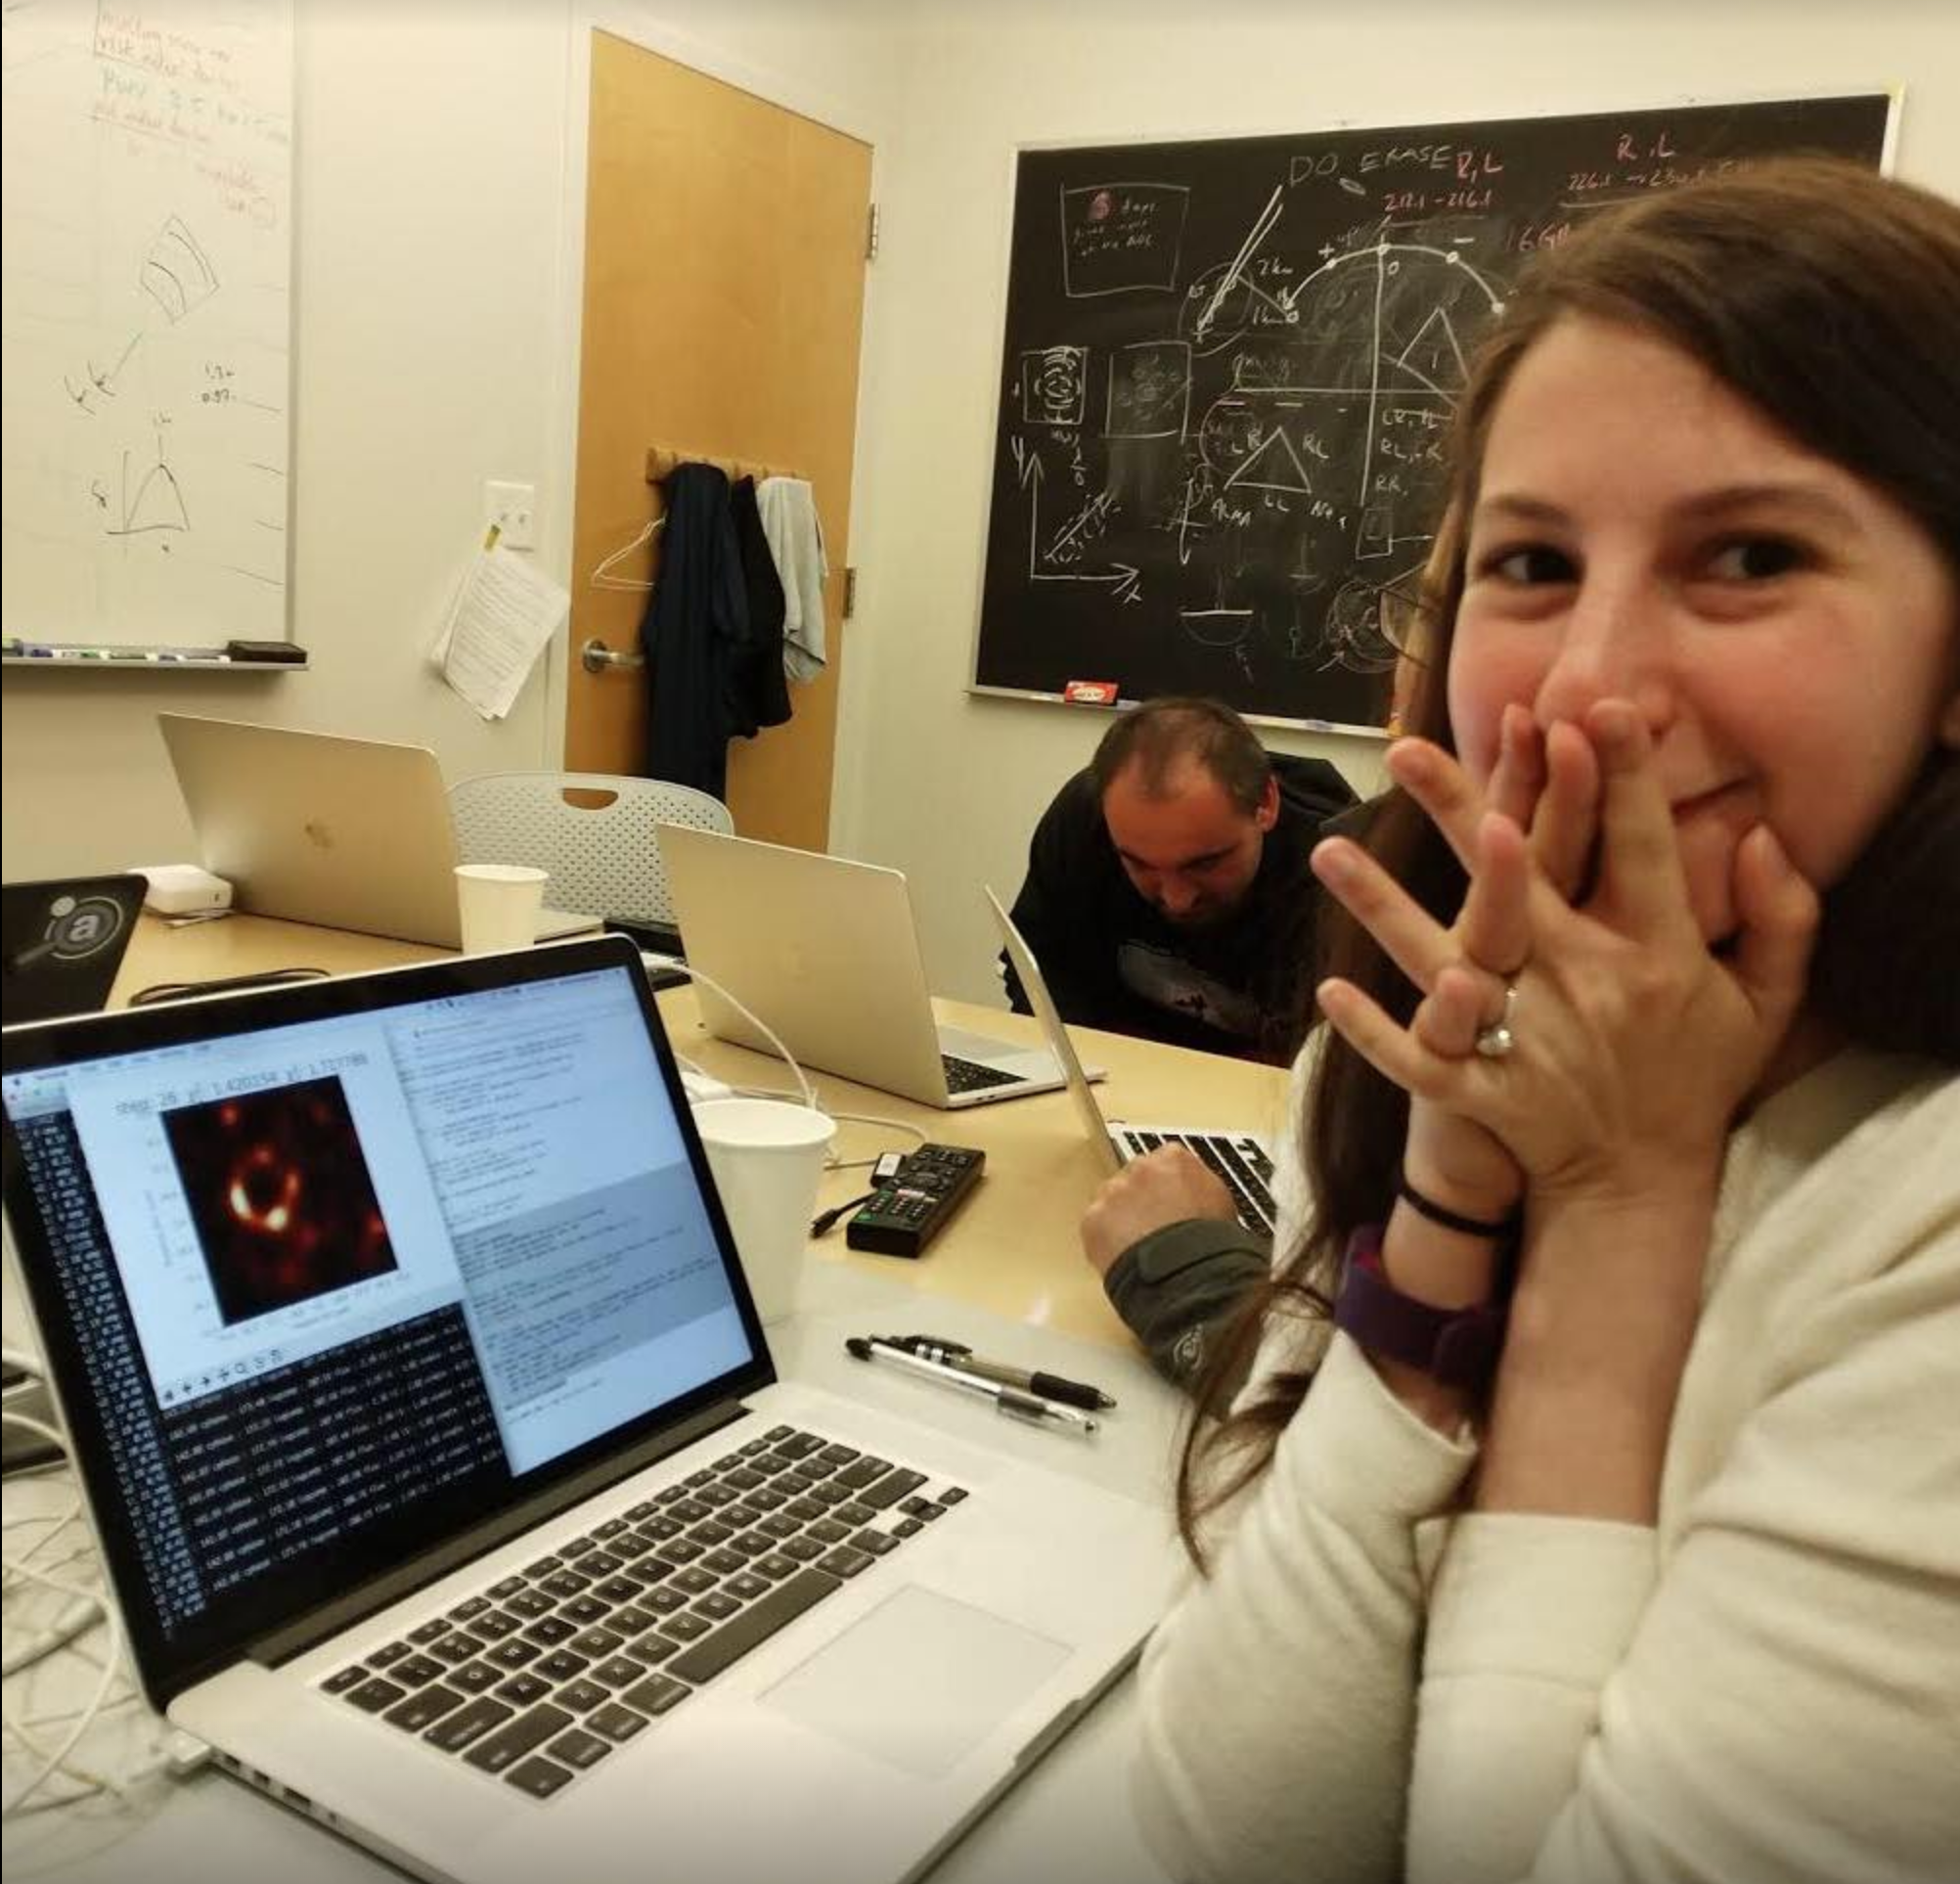
\includegraphics[width=3.98958in,height=\textheight,keepaspectratio]{index_files/mediabag/a1cd57e2943a4dd49146.png}

}

\caption{\label{fig-result-dataset}Cómo Katie Bouman se convirtió
accidentalmente en el rostro del proyecto del agujero negro.}

\end{figure}%

\section{3.2 Evidence for Multi-Reservoir
System}\label{evidence-for-multi-reservoir-system}

Our comprehensive analysis reveals three distinct seismic signatures
that strongly support the proposed multi-reservoir magma system:

\section{3.3 Pre-Eruptive Shallow Swarm
Activity}\label{pre-eruptive-shallow-swarm-activity}

Intense earthquake swarms occurred in the shallow subsurface
(\textless{} 10 km depth) during the weeks preceding the September 19th
eruption onset. This activity correlates with significant surface
deformation measurements and indicates shallow magma intrusion processes
.

\section{3.4 Syn- and Post-Eruptive Crustal Reservoir
Activity}\label{syn--and-post-eruptive-crustal-reservoir-activity}

Following eruption initiation, continuous moderate-magnitude seismicity
established at 10-15 km depth, consistent with ongoing magma movement
within the proposed shallow crustal reservoir. This persistent activity
suggests active magma storage and transport processes {[}4{]}.

\section{3.5 Deep Mantle Reservoir
Signatures}\label{deep-mantle-reservoir-signatures}

High-magnitude seismic events (M \textgreater{} 4.0) occurred
systematically at 30-40 km depths throughout the study period
\textbf{?@fig-radar}. These deeper events, while less frequent than
shallow activity, demonstrate continuous activity within the proposed
deep mantle reservoir system.

\begin{Shaded}
\begin{Highlighting}[]
\NormalTok{//| echo: false}
\NormalTok{//| label: fig{-}radar}
\NormalTok{//| fig{-}cap: "Gráfico radar de 30 indicadores de resiliencia comunitaria. Lorem ipsum dolor sit amet, consectetur adipiscing elit. Praesent tincidunt, arcu vitae suscipit commodo.Lorem ipsum dolor sit amet, consectetur adipiscing elit. Praesent tincidunt, arcu vitae suscipit commodo"}
\NormalTok{// Datos: 30 indicadores con su valor (aquí puse valores ficticios que puedes reemplazar)}
\NormalTok{data = [}
\NormalTok{  \{axis: "1. Evaluación comunitaria", value: 1.2\},}
\NormalTok{  \{axis: "2. Evaluación científica del riesgo", value: 2.0\},}
\NormalTok{  \{axis: "3. Diseminación de información en RRD", value: 2.5\},}
\NormalTok{  \{axis: "4. Educación de los niños en RRD", value: 3.0\},}
\NormalTok{  \{axis: "5. RRD en la planificación del desarrollo", value: 1.8\},}
\NormalTok{  \{axis: "6. RRD en la planificación territorial", value: 2.0\},}
\NormalTok{  \{axis: "7. Toma comunitaria de decisiones", value: 2.2\},}
\NormalTok{  \{axis: "8. Inclusión de grupos vulnerables", value: 1.7\},}
\NormalTok{  \{axis: "9. Participación de las mujeres", value: 2.3\},}
\NormalTok{  \{axis: "10. Conocimiento de derechos", value: 1.9\},}
\NormalTok{  \{axis: "11. Alianzas para la RRD", value: 2.6\},}
\NormalTok{  \{axis: "12. Gestión ambiental sostenible", value: 2.1\},}
\NormalTok{  \{axis: "13. Seguridad y gestión del agua", value: 1.8\},}
\NormalTok{  \{axis: "14. Acceso y conciencia de la salud", value: 1.6\},}
\NormalTok{  \{axis: "15. Suministro seguro de alimentos", value: 1.4\},}
\NormalTok{  \{axis: "16. Prácticas de medios de vida", value: 1.3\},}
\NormalTok{  \{axis: "17. Acceso a mercado", value: 1.5\},}
\NormalTok{  \{axis: "18. Acceso a servicios financieros", value: 1.2\},}
\NormalTok{  \{axis: "19. Protección de ingresos y activos", value: 1.7\},}
\NormalTok{  \{axis: "20. Acceso a protección social", value: 2.0\},}
\NormalTok{  \{axis: "21. Cohesión social", value: 3.2\},}
\NormalTok{  \{axis: "22. Infraestructura crítica", value: 2.8\},}
\NormalTok{  \{axis: "23. Vivienda", value: 1.9\},}
\NormalTok{  \{axis: "24. Planificación de contingencia", value: 2.1\},}
\NormalTok{  \{axis: "25. Sistema de alerta temprana", value: 2.3\},}
\NormalTok{  \{axis: "26. Capacidad de preparación", value: 2.0\},}
\NormalTok{  \{axis: "27. Servicios de salud", value: 2.5\},}
\NormalTok{  \{axis: "28. Servicios de educación", value: 2.9\},}
\NormalTok{  \{axis: "29. Infraestructura en emergencias", value: 2.7\},}
\NormalTok{  \{axis: "30. Liderazgo y voluntariado", value: 3.0\}}
\NormalTok{]}

\NormalTok{// Radar chart con D3}
\NormalTok{\{}
\NormalTok{  const width = 550, height = 550;}
\NormalTok{  const radius = Math.min(width, height) / 2 {-} 60;}
\NormalTok{  const levels = 5; // número de círculos concéntricos}
\NormalTok{  const maxValue = 3.5; // escala máxima}

\NormalTok{  const angleSlice = (Math.PI * 2) / data.length;}

\NormalTok{  const rScale = d3.scaleLinear()}
\NormalTok{    .domain([0, maxValue])}
\NormalTok{    .range([0, radius]);}

\NormalTok{  const svg = d3.create("svg")}
\NormalTok{    .attr("width", width)}
\NormalTok{    .attr("height", height);}

\NormalTok{  const g = svg.append("g")}
\NormalTok{    .attr("transform", \textasciigrave{}translate($\{width/2\},$\{height/2\})\textasciigrave{});}

\NormalTok{  // Dibujar círculos concéntricos}
\NormalTok{  for (let i = 0; i \textless{}= levels; i++) \{}
\NormalTok{    g.append("circle")}
\NormalTok{      .attr("r", radius/levels * i)}
\NormalTok{      .attr("fill", "none")}
\NormalTok{      .attr("stroke", "\#ccc");}
\NormalTok{  \}}

\NormalTok{  // Ejes radiales}
\NormalTok{  data.forEach((d, i) =\textgreater{} \{}
\NormalTok{    const angle = angleSlice * i {-} Math.PI/2;}
\NormalTok{    g.append("line")}
\NormalTok{      .attr("x1", 0)}
\NormalTok{      .attr("y1", 0)}
\NormalTok{      .attr("x2", rScale(maxValue) * Math.cos(angle))}
\NormalTok{      .attr("y2", rScale(maxValue) * Math.sin(angle))}
\NormalTok{      .attr("stroke", "\#999");}

\NormalTok{    // Etiquetas}
\NormalTok{    g.append("text")}
\NormalTok{      .attr("x", (rScale(maxValue + 0.2)) * Math.cos(angle))}
\NormalTok{      .attr("y", (rScale(maxValue + 0.2)) * Math.sin(angle))}
\NormalTok{      .attr("dy", "0.35em")}
\NormalTok{      .style("font{-}size", "10px")}
\NormalTok{      .style("text{-}anchor", angle \textgreater{} Math.PI/2 \&\& angle \textless{} 3*Math.PI/2 ? "end" : "start")}
\NormalTok{      .text(d.axis);}
\NormalTok{  \});}

\NormalTok{  // Línea de valores}
\NormalTok{  const line = d3.lineRadial()}
\NormalTok{    .radius(d =\textgreater{} rScale(d.value))}
\NormalTok{    .angle((d,i) =\textgreater{} i * angleSlice)}
\NormalTok{    .curve(d3.curveLinearClosed);}

\NormalTok{  g.append("path")}
\NormalTok{    .datum(data)}
\NormalTok{    .attr("d", line)}
\NormalTok{    .attr("fill", "rgba(50,150,250,0.5)")}
\NormalTok{    .attr("stroke", "steelblue")}
\NormalTok{    .attr("stroke{-}width", 2);}

\NormalTok{  return svg.node();}
\NormalTok{\}}
\end{Highlighting}
\end{Shaded}

\bookmarksetup{startatroot}

\chapter{4. DISCUSIÓN}\label{discusiuxf3n}

\section{4.1 Validation of Multi-Reservoir
Models}\label{validation-of-multi-reservoir-models}

The seismic evidence presented strongly validates theoretical
multi-reservoir magma storage models previously proposed for Cumbre
Vieja. The bimodal depth distribution of earthquakes, with distinct
clustering at shallow (10-15 km) and deep (30-40 km) levels, provides
compelling observational support for hierarchical magma storage systems
{[}5{]}.

\section{4.2 Implications for Volcanic Hazard
Assessment}\label{implications-for-volcanic-hazard-assessment}

Understanding magma reservoir architecture has direct implications for
eruption forecasting:

\begin{itemize}
\tightlist
\item
  \textbf{Deep reservoir monitoring}: High-magnitude events at mantle
  depths may serve as long-term eruption precursors
\item
  \textbf{Shallow reservoir dynamics}: Swarm activity in the crustal
  reservoir provides short-term eruption warnings
\item
  \textbf{System connectivity}: Temporal relationships between deep and
  shallow activity indicate reservoir interaction
\end{itemize}

\section{4.3 Methodological Advances}\label{methodological-advances}

This study demonstrates the effectiveness of systematic seismic catalog
analysis for validating geophysical models. The integration of spatial,
temporal, and magnitude characteristics provides a robust framework for
magma system characterization.

\bookmarksetup{startatroot}

\chapter{5. CONCLUSIONES}\label{conclusiones}

Analysis of 5,465 seismic events from the 2021 La Palma eruption
provides unprecedented insight into active volcanic processes:

\begin{tcolorbox}[enhanced jigsaw, rightrule=.15mm, colframe=quarto-callout-important-color-frame, opacityback=0, arc=.35mm, bottomrule=.15mm, toprule=.15mm, breakable, colback=white, leftrule=.75mm, left=2mm]

Puntos Clave

\begin{itemize}
\tightlist
\item
  Lorem ipsum dolor sit amet, consectetur adipiscing elit. Praesent
  tincidunt, arcu vitae suscipit commodo.
\item
  Lorem ipsum dolor sit amet, consectetur adipiscing elit. Praesent
  tincidunt, arcu vitae suscipit commodo.
\item
  Lorem ipsum dolor sit amet, consectetur adipiscing elit. Praesent
  tincidunt, arcu vitae suscipit commodo.
\end{itemize}

\end{tcolorbox}

\begin{tcolorbox}[enhanced jigsaw, rightrule=.15mm, colframe=quarto-callout-important-color-frame, opacityback=0, arc=.35mm, bottomrule=.15mm, toprule=.15mm, breakable, colback=white, leftrule=.75mm, left=2mm]

Preguntas por resolver

\begin{itemize}
\tightlist
\item
  Lorem ipsum dolor sit amet, consectetur adipiscing elit. Praesent
  tincidunt, arcu vitae suscipit commodo.
\item
  Lorem ipsum dolor sit amet, consectetur adipiscing elit. Praesent
  tincidunt, arcu vitae suscipit commodo.
\item
  Lorem ipsum dolor sit amet, consectetur adipiscing elit. Praesent
  tincidunt, arcu vitae suscipit commodo.
\end{itemize}

\end{tcolorbox}

\begin{tcolorbox}[enhanced jigsaw, rightrule=.15mm, colframe=quarto-callout-important-color-frame, opacityback=0, arc=.35mm, bottomrule=.15mm, toprule=.15mm, breakable, colback=white, leftrule=.75mm, left=2mm]

Recomendaciones para tomar decisiones

\begin{itemize}
\tightlist
\item
  Lorem ipsum dolor sit amet, consectetur adipiscing elit. Praesent
  tincidunt, arcu vitae suscipit commodo.
\item
  Lorem ipsum dolor sit amet, consectetur adipiscing elit. Praesent
  tincidunt, arcu vitae suscipit commodo.
\item
  Lorem ipsum dolor sit amet, consectetur adipiscing elit. Praesent
  tincidunt, arcu vitae suscipit commodo.
\end{itemize}

\end{tcolorbox}

\bookmarksetup{startatroot}

\chapter{AGRADECIMIENTOS}\label{agradecimientos}

Lorem ipsum dolor sit amet, consectetur adipiscing elit. Praesent
tincidunt, arcu vitae suscipit commodo. Lorem ipsum dolor sit amet,
consectetur adipiscing elit. Praesent tincidunt, arcu vitae suscipit
commodo. Lorem ipsum dolor sit amet, consectetur adipiscing elit.
Praesent tincidunt, arcu vitae suscipit commodo.

\bookmarksetup{startatroot}

\chapter{DECLARACIÓN DE AUTORIA
CREDIT}\label{declaraciuxf3n-de-autoria-credit}

Seismic data were obtained from the Instituto Geográfico Nacional (IGN)
public database. Data processing scripts, analysis notebooks, and
visualization tools have been developed to ensure reproducibility and
are available through institutional repositories. All methodological
approaches follow open science principles to facilitate community
validation and extension.

\bookmarksetup{startatroot}

\chapter{BIBLIOGRAFÍA}\label{bibliografuxeda}

\phantomsection\label{refs}
\begin{CSLReferences}{0}{1}
\bibitem[\citeproctext]{ref-connor2015}
\CSLLeftMargin{1. }%
\CSLRightInline{Connor C, Bebbington M, Marzocchi W. Probabilistic
Volcanic Hazard Assessment {[}Internet{]}. Elsevier Inc.; 2015.
Disponible en:
\url{http://dx.doi.org/10.1016/B978-0-12-385938-9.00051-1}}

\bibitem[\citeproctext]{ref-lindsay2018}
\CSLLeftMargin{2. }%
\CSLRightInline{Lindsay JM, Robertson REA.
\href{https://doi.org/10.3389/feart.2018.00042}{Integrating volcanic
hazard data in a systematic approach to develop volcanic hazard maps in
the lesser antilles}. Frontiers in Earth Science. 2018;6(April):1-17. }

\bibitem[\citeproctext]{ref-jenkins2014}
\CSLLeftMargin{3. }%
\CSLRightInline{Jenkins SF, Spence RJS, Fonseca JFBD, Solidum RU, Wilson
TM. Volcanic risk assessment: Quantifying physical vulnerability in the
built environment. Journal of Volcanology and Geothermal Research
{[}Internet{]}. 2014;276:105-20. Disponible en:
\url{http://dx.doi.org/10.1016/j.jvolgeores.2014.03.002}}

\bibitem[\citeproctext]{ref-woodford2015}
\CSLLeftMargin{4. }%
\CSLRightInline{Woodford KO. Global volcanic hazards and risk. 2015. }

\bibitem[\citeproctext]{ref-williams-jones2015}
\CSLLeftMargin{5. }%
\CSLRightInline{Williams-Jones G, Rymer H. Hazards of Volcanic Gases
{[}Internet{]}. Elsevier Inc.; 2015. Disponible en:
\url{http://dx.doi.org/10.1016/B978-0-12-385938-9.00057-2}}

\bibitem[\citeproctext]{ref-narvaez2009}
\CSLLeftMargin{6. }%
\CSLRightInline{Narváez L, Lavell A, Pérez Ortega G. La gestión del
riesgo de desastres: Un enfoque basado en procesos {[}Internet{]}.
Comunidad Andina; 2009. Disponible en:
\url{http://www.comunidadandina.org/predecan/doc/libros/PROCESOS_ok.pdf}}

\bibitem[\citeproctext]{ref-torrico2008}
\CSLLeftMargin{7. }%
\CSLRightInline{Torrico Canaviri G, Ortiz Cañipa S, Salamanca Mazuelo
LA, Quiroga Becerra de la Roca R. Los enfoques teóricos del desastre y
la gestión local del riesgo: Construcción crítica del concepto. National
Centre of Competence in Research North-South (NCCR); OXFAM; Fundación
para el Desarrollo Participativo Comunitario (FUNDEPCO); 2008. }

\bibitem[\citeproctext]{ref-maskrey1998}
\CSLLeftMargin{8. }%
\CSLRightInline{Maskrey A. Navegando entre brumas: La aplicación de los
sistemas de información geográfica al análisis de riesgo en América
Latina {[}Internet{]}. Red de Estudios Sociales en Prevención de
Desastres en América Latina; 1998. Disponible en:
\url{https://www.desenredando.org/public/libros/1998/neb/neb_intro_nov-09-2002.pdf}}

\bibitem[\citeproctext]{ref-alcantara2025}
\CSLLeftMargin{9. }%
\CSLRightInline{Alcántara-Ayala I. Cascading hazards and compound
disasters. NPJ Natural Hazards {[}Internet{]}. 2025;2(1). Disponible en:
\url{https://doi.org/10.1038/s44304-025-00111-5}}

\bibitem[\citeproctext]{ref-commoner1973}
\CSLLeftMargin{10. }%
\CSLRightInline{Commoner B. El círculo que se cierra. Plaza \& Janés;
1973. }

\bibitem[\citeproctext]{ref-capra2014}
\CSLLeftMargin{11. }%
\CSLRightInline{Capra F, Luisi PL. The systems view of life: A unifying
vision {[}Internet{]}. Cambridge University Press; 2014. Disponible en:
\url{https://doi.org/10.1017/CBO9780511895555}}

\bibitem[\citeproctext]{ref-spivak2003}
\CSLLeftMargin{12. }%
\CSLRightInline{Chakravorty Spivak G, Giraldo S. ¿Puede hablar el
subalterno? Revista Colombiana de Antropología {[}Internet{]}.
2003;297-364. Disponible en:
\url{https://doi.org/10.22380/2539472X.1244}}

\bibitem[\citeproctext]{ref-hallegatte2017}
\CSLLeftMargin{13. }%
\CSLRightInline{Hallegatte S, Vogt-Schilb A, Bangalore M, Rozenberg J.
Unbreakable: Building the resilience of the poor in the face of natural
disasters {[}Internet{]}. The World Bank; 2017. Disponible en:
\url{http://documents1.worldbank.org/curated/en/512241480487839624/pdf/Unbreakable-building-the-resilience-of-the-poor-in-the-face-of-natural-disasters.pdf}}

\bibitem[\citeproctext]{ref-ley1523}
\CSLLeftMargin{14. }%
\CSLRightInline{Congreso de Colombia. Ley 1523: Por la cual se adopta la
política nacional de gestión del riesgo de desastres y se establece el
Sistema Nacional de Gestión del Riesgo de Desastres y se dictan otras
disposiciones. Bogotá D.C.; 2012. }

\bibitem[\citeproctext]{ref-montero2004}
\CSLLeftMargin{15. }%
\CSLRightInline{Montero M. Introducción a la psicología comunitaria:
Desarrollo, conceptos y procesos. Paidós; 2004. }

\bibitem[\citeproctext]{ref-navarro2020}
\CSLLeftMargin{16. }%
\CSLRightInline{Navarro Martínez SI. Discursos y prácticas de la
educación superior intercultural: La experiencia de Chiapas
{[}Internet{]}. CLACSO; 2020. Disponible en:
\url{https://biblioteca.clacso.edu.ar/clacso/se/20201124055040/Discursos-y-practicas.pdf}}

\bibitem[\citeproctext]{ref-sanchez2013}
\CSLLeftMargin{17. }%
\CSLRightInline{Sánchez Teruel D, Robles Bello MA. Inclusión como clave
de una educación para todos: Revisión teórica. Revista Española de
Orientación y Psicopedagogía {[}Internet{]}. 2013;24-36. Disponible en:
\url{https://doi.org/10.5944/reop.vol.24.num.2.2013.11257}}

\bibitem[\citeproctext]{ref-ungrd2016}
\CSLLeftMargin{18. }%
\CSLRightInline{Unidad Nacional para la Gestión del Riesgo de Desastres
(UNGRD). Plan Nacional de Gestión del Riesgo de Desastres: Una
estrategia de desarrollo 2015--2025 {[}Internet{]}. Unidad Nacional para
la Gestión del Riesgo de Desastres; 2016. Disponible en:
\url{https://portal.gestiondelriesgo.gov.co/Paginas/Plan-Nacional-de-Gestion-del-Riesgo.aspx}}

\bibitem[\citeproctext]{ref-rodriguez2016}
\CSLLeftMargin{19. }%
\CSLRightInline{Rodríguez AR, Montenegro M. Retos contemporáneos para la
psicología comunitaria: Reflexiones sobre la noción de comunidad.
Interamerican Journal of Psychology {[}Internet{]}. 2016;14-22.
Disponible en: \url{https://doi.org/10.30849/rip/ijp.v50i1.40}}

\bibitem[\citeproctext]{ref-guzman2020}
\CSLLeftMargin{20. }%
\CSLRightInline{Guzmán-Valenzuela C, Rojas-Murphy Tagle A,
Gómez-González C. Epistemic polyphony of research on the students'
experiences: The Latin-American case. Education Policy Analysis Archives
{[}Internet{]}. 2020;28:96. Disponible en:
\url{https://doi.org/10.14507/epaa.28.4919}}

\bibitem[\citeproctext]{ref-lastra2020}
\CSLLeftMargin{21. }%
\CSLRightInline{Lastra MS. Polifonía política de los retornos del
exilio: Reflexiones y preguntas desde el Cono Sur. En: Coraza de los
Santos E, Lastra S, editores. Miradas a las migraciones, las fronteras y
los exilios {[}Internet{]}. Consejo Latinoamericano de Ciencias
Sociales; 2020. p. 175-95. Disponible en:
\url{http://hdl.handle.net/11336/192669}}

\bibitem[\citeproctext]{ref-sciurano2022}
\CSLLeftMargin{22. }%
\CSLRightInline{Sciurano GA, Melamud M. ¿Ellos o nosotros? Escritura
polifónica y los límites del campo en un estudio etnográfico sobre
nuevas espiritualidades. Campos: Revista de Antropología Social
{[}Internet{]}. 2022;23(1):222-47. Disponible en:
\url{https://doi.org/10.5380/cra.v23i1.82198}}

\bibitem[\citeproctext]{ref-reales2022}
\CSLLeftMargin{23. }%
\CSLRightInline{Reales Chacón L, Robalino Morales G, Peñafiel Luna A,
Cárdenas Medina J, Cantuña-Vallejo P. El muestreo intencional no
probabilístico como herramienta de la investigación científica en
carreras de ciencias de la salud. Universidad y Sociedad {[}Internet{]}.
2022;14(S5):681-91. Disponible en:
\url{https://rus.ucf.edu.cu/index.php/rus/article/view/3338}}

\bibitem[\citeproctext]{ref-giesecke2020}
\CSLLeftMargin{24. }%
\CSLRightInline{Giesecke Sara Lafosse MP. Elaboración y pertinencia de
la matriz de consistencia cualitativa para las investigaciones en
ciencias sociales. Desde el Sur {[}Internet{]}. 2020;12(2):397-417.
Disponible en: \url{https://doi.org/10.21142/des-1202-2020-0023}}

\bibitem[\citeproctext]{ref-alaggia2020}
\CSLLeftMargin{25. }%
\CSLRightInline{Alaggia R, Wang S. I never told anyone until the \#metoo
movement: What can we learn from sexual abuse and sexual assault
disclosures made through social media? Child Abuse \& Neglect
{[}Internet{]}. 2020;103:104312. Disponible en:
\url{https://doi.org/10.1016/j.chiabu.2019.104312}}

\bibitem[\citeproctext]{ref-humanity2020}
\CSLLeftMargin{26. }%
\CSLRightInline{Humanity \& Inclusion. Estudio de diagnóstico de la
integración de la inclusión y la protección en el plan nacional de
gestión del riesgo de desastres en Colombia. Humanity \& Inclusion
Colombia; 2020. }

\bibitem[\citeproctext]{ref-ungrd2019}
\CSLLeftMargin{27. }%
\CSLRightInline{Unidad Nacional para la Gestión del Riesgo de Desastres.
El enfoque diferencial en la gestión del riesgo de desastres: etnia,
género y discapacidad {[}Internet{]}. 2019. Disponible en:
\url{https://portal.gestiondelriesgo.gov.co/Documents/ENFOQUE-DIFERENCIAL-Y-DE-GENERO-UNGRD.pdf}}

\bibitem[\citeproctext]{ref-ungrd2017}
\CSLLeftMargin{28. }%
\CSLRightInline{Unidad Nacional para la Gestión del Riesgo de Desastres.
Guía para la participación comunitaria en la gestión del riesgo de
desastres {[}Internet{]}. 2017. Disponible en:
\url{http://repositorio.gestiondelriesgo.gov.co/handle/20.500.11762/20793}}

\bibitem[\citeproctext]{ref-ungrd2013}
\CSLLeftMargin{29. }%
\CSLRightInline{Unidad Nacional para la Gestión del Riesgo de Desastres.
Guía comunitaria para la gestión del riesgo de desastre {[}Internet{]}.
2013. Disponible en:
\url{https://repositorio.gestiondelriesgo.gov.co:8443/bitstream/handle/20.500.11762/157/2-guia-comunitaria-grd.pdf}}

\bibitem[\citeproctext]{ref-amorim2022}
\CSLLeftMargin{30. }%
\CSLRightInline{Amorim-Maia AT, Anguelovski I, Chu E, Connolly J.
Intersectional climate justice: A conceptual pathway for bridging
adaptation planning, transformative action, and social equity. Urban
Climate {[}Internet{]}. 2022;41:101053. Disponible en:
\url{https://doi.org/10.1016/j.uclim.2021.101053}}

\bibitem[\citeproctext]{ref-andreucci2022}
\CSLLeftMargin{31. }%
\CSLRightInline{Andreucci D, Zografos C. Between improvement and
sacrifice: Othering and the (bio)political ecology of climate change.
Political Geography {[}Internet{]}. 2022;92:102512. Disponible en:
\url{https://doi.org/10.1016/j.polgeo.2021.102512}}

\bibitem[\citeproctext]{ref-eriksen2021}
\CSLLeftMargin{32. }%
\CSLRightInline{Eriksen S, Schipper ELF, Scoville-Simonds M, Vincent K,
Adam HN, Brooks N, et~al. Adaptation interventions and their effect on
vulnerability in developing countries: Help, hindrance or irrelevance?
World Development {[}Internet{]}. 2021;141:105383. Disponible en:
\url{https://doi.org/10.1016/j.worlddev.2020.105383}}

\bibitem[\citeproctext]{ref-diaz2025}
\CSLLeftMargin{33. }%
\CSLRightInline{Díaz Heredia LP, Medina M, Corredor Pardo KA, Gómez J.
Propuesta metodológica participativa desde Colombia para la recolección
de datos en gestión del riesgo de emergencias y desastres. Revista de
Estudios Latinoamericanos sobre Reducción del Riesgo de Desastres REDER
{[}Internet{]}. 2025;9(2):106. Disponible en:
\url{https://doi.org/10.55467/reder.v9i2.198}}

\bibitem[\citeproctext]{ref-sandoval2021}
\CSLLeftMargin{34. }%
\CSLRightInline{Sandoval-Díaz J, Martínez-Labrín S. Gestión comunitaria
del riesgo de desastre: Una propuesta metodológica-reflexiva desde las
metodologías participativas. Revista de Estudios Latinoamericanos sobre
Reducción del Riesgo de Desastres REDER {[}Internet{]}. 2021;5(2):75.
Disponible en: \url{https://doi.org/10.55467/reder.v5i2.73}}

\bibitem[\citeproctext]{ref-suazo2025}
\CSLLeftMargin{35. }%
\CSLRightInline{Suazo-Muñoz C, Sandoval-Díaz J, Navarrete-Valladares C.
Metodologías participativas en la gestión comunitaria del riesgo de
desastre: Revisión sistemática de experiencias en América Latina.
Perspectiva Geográfica {[}Internet{]}. 2025;30(2):1-21. Disponible en:
\url{https://doi.org/10.19053/uptc.01233769.18118}}

\bibitem[\citeproctext]{ref-ramirez2016}
\CSLLeftMargin{36. }%
\CSLRightInline{Ramírez Elizalde LA, Vélez Torres I. Percepción social y
respuesta institucional frente al desastre de Tierradentro, Colombia.
Perspectiva Geográfica {[}Internet{]}. 2016;20(2):269-96. Disponible en:
\url{https://doi.org/10.19053/01233769.4517}}

\bibitem[\citeproctext]{ref-hernandez2020}
\CSLLeftMargin{37. }%
\CSLRightInline{Hernández Peña YT, Vargas Cuervo G, Zafra Mejía CA.
Percepciones sobre fenómenos volcánicos: Elementos para la gestión del
riesgo en Colombia. Perspectiva Geográfica {[}Internet{]}. 2020;99-119.
Disponible en: \url{https://doi.org/10.19053/01233769.9488}}

\bibitem[\citeproctext]{ref-londono2024}
\CSLLeftMargin{38. }%
\CSLRightInline{Londoño PAV, Monsalve LFD, Trujillo SP. The significance
of prior resilience experiences in communities exposed to
socio-political violence in Colombia for enhancing the community-based
disaster management (CBDM) model. Journal of Infrastructure, Policy and
Development {[}Internet{]}. 2024;8(9):5352. Disponible en:
\url{https://doi.org/10.24294/jipd.v8i9.5352}}

\bibitem[\citeproctext]{ref-rivera2020}
\CSLLeftMargin{39. }%
\CSLRightInline{Rivera Flórez LA, Rodríguez Gaviria EM, Velásquez
Castañeda CA, Guzmán Tenjo HP, Ramírez Madrigal A. La gestión
comunitaria del riesgo: Justicia espacial y ambiental. Bitácora Urbano
Territorial {[}Internet{]}. 2020;30(3):205-18. Disponible en:
\url{https://doi.org/10.15446/bitacora.v30n3.87769}}

\bibitem[\citeproctext]{ref-valencia2024}
\CSLLeftMargin{40. }%
\CSLRightInline{Valencia Londoño PA, Valencia Londoño D. Persistent
vulnerability after disaster risk reduction (DRR) response: The case of
Salgar, Colombia. Sustainability {[}Internet{]}. 2024;16(11):4394.
Disponible en: \url{https://doi.org/10.3390/su16114394}}

\bibitem[\citeproctext]{ref-hadlos2022}
\CSLLeftMargin{41. }%
\CSLRightInline{Hadlos A, Opdyke A, Hadigheh SA. Where does local and
indigenous knowledge in disaster risk reduction go from here? A
systematic literature review. International Journal of Disaster Risk
Reduction {[}Internet{]}. 2022;79:103160. Disponible en:
\url{https://doi.org/10.1016/j.ijdrr.2022.103160}}

\bibitem[\citeproctext]{ref-vasileiou2022}
\CSLLeftMargin{42. }%
\CSLRightInline{Vasileiou K, Barnett J, Fraser DS. Integrating local and
scientific knowledge in disaster risk reduction: A systematic review of
motivations, processes, and outcomes. International Journal of Disaster
Risk Reduction {[}Internet{]}. 2022;81:103255. Disponible en:
\url{https://doi.org/10.1016/j.ijdrr.2022.103255}}

\bibitem[\citeproctext]{ref-baudoin2016}
\CSLLeftMargin{43. }%
\CSLRightInline{Baudoin M-A, Henly-Shepard S, Fernando N, Sitati A,
Zommers Z. From top-down to "community-centric" approaches to early
warning systems: Exploring pathways to improve disaster risk reduction
through community participation. International Journal of Disaster Risk
Science {[}Internet{]}. 2016;7(2):163-74. Disponible en:
\url{https://doi.org/10.1007/s13753-016-0085-6}}

\end{CSLReferences}

\bookmarksetup{startatroot}

\chapter{2. Enfoque etnodiferencial y riesgo de desastre en Colombia:
líneas de fuga para una digna
vida}\label{enfoque-etnodiferencial-y-riesgo-de-desastre-en-colombia-luxedneas-de-fuga-para-una-digna-vida}

\phantomsection\label{resumen}
\bookmarksetup{startatroot}

\chapter{Resumen}\label{resumen-1}

En Colombia, la gestión del riesgo de desastres ha reflejado la
subalternización histórica de las voces comunitarias al percibir la
diferencia cultural como un obstáculo en lugar de una potencialidad.
Este reflejo es posible en tanto se ha sostenido un orden social que
privilegia la homogenización por encima de las realidades situadas. Para
reconfigurar esta práctica relacional, es prioritario reconocer la
riqueza inherente a las comunidades. Dada la constante exposición del
país a fenómenos naturales, un enfoque que trascienda la recopilación de
datos es fundamental. Este estudio abordó las posibilidades de
articulación del enfoque etnodiferencial en la Gestión del Riesgo de
Desastres (GRD) en Colombia. Para ello, se desarrolló una investigación
de corte cualitativo que incluyó la realización de seis grupos focales y
catorce entrevistas a profundidad con representantes comunitarios e
institucionales. Estos instrumentos permitieron explorar la diversidad
de perspectivas sobre el desastre y facilitaron el surgimiento de
conocimientos arraigados en el diálogo y la interacción, visibilizando
las voces históricamente silenciadas. El principal hallazgo implica
reconocer que desmantelar la noción de subalternidad y adoptar una
visión diversa no solo conduce a una reducción del sufrimiento, sino que
también promueve la justicia, la dignidad y el reconocimiento de todas
las voces. En conclusión, la investigación demostró que el enfoque
etnodiferencial puede redefinir la GRD al centrarse en el diálogo y el
respeto por la diversidad como elementos esenciales para transformar la
relación entre las comunidades y las instituciones. Esta perspectiva
tensiona los límites tradicionales de la gestión del riesgo, abriendo el
camino hacia un proceso auténticamente humano. Se confirma que cada
cultura y experiencia comunitaria aporta un valor único al panorama
general, lo que permite una comprensión integral y una respuesta eficaz
a los desastres.

\phantomsection\label{abstract}
\bookmarksetup{startatroot}

\chapter{Ethno-differential approach and disaster risk in Colombia:
lines of flight for a dignified
life}\label{ethno-differential-approach-and-disaster-risk-in-colombia-lines-of-flight-for-a-dignified-life}

\textbf{Abstract}. In Colombia, disaster risk management has reflected
the historical subalternization of community voices by perceiving
cultural difference as an obstacle rather than a potentiality. This
reflection is possible insofar as a social order has been sustained that
privileges homogenization over situated realities. To reconfigure this
relational practice, recognizing the inherent richness of communities is
a priority. Given the country's constant exposure to natural phenomena,
an approach that transcends mere data collection is fundamental. This
study addressed the potential integration of the ethno-differential
approach into Disaster Risk Management (DRM) in Colombia. To this end, a
qualitative research design was developed, which included conducting six
focus groups and fourteen in-depth interviews with community and
institutional representatives. These instruments enabled the exploration
of diverse perspectives on disasters and facilitated the emergence of
knowledge rooted in dialogue and interaction, giving visibility to
historically silenced voices. The main finding underscores the
importance of dismantling the notion of subalternity and adopting a
diverse vision, which not only leads to a reduction in suffering but
also promotes justice, dignity, and the recognition of all voices. In
conclusion, the research demonstrated that the ethno-differential
approach could redefine DRM by focusing on dialogue and respect for
diversity as essential elements for transforming the relationship
between communities and institutions. This perspective challenges the
traditional boundaries of disaster risk management, paving the way for a
genuinely human process. It is confirmed that each culture and community
experience contributes a unique value to the broader picture, enabling a
comprehensive understanding and an effective response to disasters.

\bookmarksetup{startatroot}

\chapter{1. INTRODUCCIÓN}\label{introducciuxf3n-1}

El desastre es una ruptura de la cotidianidad. En un territorio
específico, las interacciones socioambientales que se han venido
configurando se fracturan, lo que genera un profundo sufrimiento para el
cuerpo subjetivo, político y territorial. Evitar este dolor representa
un acto de justicia con la digna vida, en tanto aquel padecimiento es
evitable. Así, en clave de promoción de la digna vida y evitación de
sufrimientos emerge la gestión del riesgo de desastres (GRD), concebida
como un proceso social orientado a la transformación de las relaciones
entre los seres humanos y la naturaleza {[}6{]}.

Ahora bien, aun cuando su horizonte es loable, la GRD se ha visto
inmersa en una tensión discursiva desde hace varios años. Por un lado,
encontramos el enfoque que comprende el desastre desde una perspectiva
fisicalista, que privilegia el estudio de las amenazas por encima de
cualquier otro factor {[}7{]}. Por otro lado, existen los planteamientos
construccionistas, que interpretan el riesgo y el desastre como
fenómenos emergentes de la compleja red de interacciones humanas
{[}8,9{]}.

Esta tensión no es menor, en tanto el ángulo de colocación-acción que
soportan determinará los procesos que han de llevarse a cabo. Al elegir
una visión fisicalista, se podría desatender el diálogo sobre el
desarrollo social, aunque se logren avances significativos en la
comprensión de los procesos naturales subyacentes. En contraste, optar
por un enfoque construccionista puede llevar a una menor atención a los
procesos físicos, pero proporciona un marco más rico para entender
cuestiones de desigualdad social, exclusión, segregación, vulnerabilidad
y desarrollo de capacidades.

Esta divergencia en los enfoques resalta la complejidad inherente al
riesgo y al desastre, que son fenómenos multifacéticos y no lineales.
Indistintamente del enfoque que se elija, no puede perderse de vista el
horizonte de digna vida tanto para los seres humanos como para aquellos
que no. La GRD implica un marco de enunciación ético-político en defensa
de la vida. Este contexto invita al reconocimiento de sus múltiples
tramas y a la necesidad de diálogos interdisciplinarios para abordar el
problema de manera integral {[}10,11{]}.

Sin embargo, el desarrollo de un diálogo significativo es posible solo
cuando todos los participantes tienen igual relevancia en el discurso.
Lamentablemente, esta igualdad no siempre se logra, como lo señaló
Spivak al afirmar: ``el subalterno no es un sujeto que ocupa una
posición discursiva desde la que puede hablar o responder {[}\ldots{]}
es el espacio en blanco entre las palabras; el hecho de que se le
silencie no significa que no exista'' {[}12{]}.

La noción de subalterno subraya el reconocimiento de grupos sociales que
históricamente han sido silenciados e ignorados, pero que, como lo ha
demostrado la investigación, son los más afectados por los desastres.
Mujeres, comunidades diversas sexual y funcionalmente,
afrodescendientes, indígenas, personas con bajos ingresos económicos y
quienes tienen un acceso limitado a servicios públicos {[}13{]}
constituyen estos intersticios discursivos, ausentes en la polifonía de
la GRD.

A partir de esta premisa, la GRD no puede considerarse un proceso social
si se soporta en exclusiones, segregaciones o silenciamientos, lo cual
ha sido naturalizado en las expresiones cotidianas: ``el trabajo con
comunidades es difícil, es que las comunidades son problemáticas, es
necesario desarrollar conocimiento para las comunidades.'' De plano,
este tipo de configuraciones discursivas parte de la negación epistémica
de otro que se expresa de forma diferente a la habitual, convoca un
silenciamiento y una verticalización del poder, en tanto el acercamiento
comunitario parte de la desconfianza y desdén. Por esta razón, referirse
a un enfoque etnodiferencial en la GRD es un llamado de atención ante la
práctica persistente de silenciar voces.

\begin{tcolorbox}[enhanced jigsaw, rightrule=.15mm, colframe=quarto-callout-important-color-frame, opacityback=0, arc=.35mm, bottomrule=.15mm, toprule=.15mm, breakable, colback=white, leftrule=.75mm, left=2mm]

Caja 1. Avances en Colombia hacia una GRD participativa, inclusiva y
diversa

En Colombia, se ha intentado avanzar hacia una GRD participativa,
inclusiva y diversa. Dos instrumentos jurídico-políticos de relevancia
lo demuestran. El primero es la Ley 1523 de 2012, mediante la cual se
adopta la política nacional de gestión del riesgo de desastres y se
establece el Sistema Nacional de Gestión del Riesgo de Desastres
{[}14{]}. En su artículo 3ro, se definen los principios generales de la
GRD. Entre estos principios, destacan dos que son relevantes para
nuestro análisis.

\textbf{Principio participativo.} Es deber de las autoridades y
entidades del Sistema Nacional de Gestión del Riesgo de Desastres,
reconocer, facilitar y promover la organización y participación de
comunidades étnicas, asociaciones cívicas, comunitarias, vecinales,
benéficas, de voluntariado y de utilidad común. Es deber de todas las
personas hacer parte del proceso de gestión del riesgo en su comunidad.

\textbf{Principio de diversidad cultural.} En reconocimiento de los
derechos económicos, sociales y culturales de las personas, los procesos
de la gestión del riesgo deben ser respetuosos de las particularidades
culturales de cada comunidad y aprovechar al máximo los recursos
culturales de la misma.

\end{tcolorbox}

Con base en estos principios, solo existe un camino viable para la GRD:
uno que centre su acción en las realidades y voces de las comunidades.
De acuerdo con Montero {[}15{]}, ``lo comunitario incluye el rol activo
de la comunidad, su participación. Y no sólo como invitada, o como
espectadora aceptada o receptora de beneficios, sino como agente activo
con voz, voto y veto'' (p.~31).

Desde esta perspectiva, el enfoque etnodiferencial en la GRD requiere el
conocimiento y reconocimiento de la diversidad, no como una forma de
clasificar comportamientos, sino como una apuesta por lo común, por el
encuentro con el otro en contextos de incertidumbre y la aceptación de
su humanidad {[}16,17{]}.

El segundo instrumento jurídico-político relevante es el Plan Nacional
de Gestión del Riesgo de Desastres ``Una estrategia de Desarrollo''
2015-2025 {[}18{]}. En este plan, se establece como objetivo estratégico
fortalecer la gobernanza, la educación y la comunicación social en la
gestión del riesgo, con un enfoque diferencial, de género y de
diversidad cultural. Al respecto, se señala:

El trabajo con comunidades será respetuoso del enfoque diferencial,
considerando los valores culturales, religiosos y sociales, y no debe
existir discriminación de ningún tipo en las acciones que el Sistema
Nacional de Gestión del Riesgo (SNGRD) impulse en el territorio
nacional, especialmente en relación con edad, sexo, condición social,
etnias y grupos minoritarios, población indígena y comunidades
afrodescendientes, y personas en situación de discapacidad (pág. 31).

En este marco, el reconocimiento de las realidades y voces comunitarias,
así como su participación dialógica, conlleva al fortalecimiento de la
gobernanza, la educación y la comunicación social. El objetivo es
favorecer la expresión de comunidades vivas y activas, capaces de
gestionar su propio entorno, en consonancia con Rodríguez y Montenegro
{[}19{]}:

La toma de decisiones es la manera en que la comunidad puede vivirse, la
forma en que estamos con los otros u otras. He aquí, en el tratamiento
de la diferencia y de la posibilidad del encuentro, donde reside el
componente político y ético de lo que entendemos por comunidad (pág.
16).

Por lo tanto, la incorporación del enfoque etnodiferencial en la GRD
convoca a explorar sus posibilidades de articulación ---propósito de
esta investigación---. Esta incorporación precisa ser vista como
ejercicio ontológico dado que busca superar la subalternidad que
históricamente ha caracterizado a muchas comunidades, permitiendo un
reconocimiento de estas como agentes activos en la construcción de su
propio mundo y como praxis transformadora en cuanto se orienta hacia la
reducción de riesgos y desastres mediante el diálogo entre saberes,
acciones y poderes.

\bookmarksetup{startatroot}

\chapter{2. METODOLOGÍA}\label{metodologuxeda}

La investigación adelantada fue de tipo cualitativa, estructurada
mediante fases polifónicas. Esta noción hace referencia a estadios de
diálogo que reúnen diversas voces, permitiendo que emerja un discurso
generativo {[}20,21{]} en clave de las categorías etnodiferencial y GRD,
seguidas por la pregunta amplia: ¿Cuáles son las posibilidades de
articulación del enfoque etnodiferencial a la GRD en Colombia? Estas
fases se complementaron con un proceso de acuerdos narrativos {[}22{]},
mediante el cual se armonizan los tonos discursivos y operativos en
colaboración con las instancias responsables del proyecto. En
consecuencia, las fases polifónicas se desarrollaron de la siguiente
manera:

\textbf{Fase polifónica I.} Esta fase implicó la revisión de documentos
sobre el enfoque etnodiferencial en la GRD en Latinoamérica, con énfasis
en Colombia. Se exploraron Google Académico, Redalyc, Scielo, Ebsco,
CEPAL, Dialnet, Tesis Doctorales en Red y UNESCO, utilizando palabras
clave como ``etnodiferencial'', ``diversidad'', ``desastres'',
``riesgos'', ``recuperación'', ``rehabilitación'' y ``reconstrucción'',
en el rango temporal 2016--2021. De 213 textos iniciales, se eliminaron
duplicados y no relevantes, quedando 80; la saturación categorial redujo
la unidad de trabajo a 50. Este proceso aseguró una base sólida para
analizar el componente étnico en la GRD. La metodología de selección
aplicada refleja un enfoque transparente, alineado con los estándares de
revisión, facilitando futuras investigaciones y aplicaciones prácticas
en contextos étnicos diversos.

\textbf{Fase polifónica II.} En esta fase se desarrollaron narrativas
generativas, donde las voces de miembros de comunidades e instituciones,
sus experiencias cotidianas y sus formas de vida contribuyeron a la
construcción de líneas de fuga para la incorporación del enfoque
diferencial en la gestión del riesgo de desastres. Este proceso incluyó:
6 grupos focales en modalidad virtual (3 con instituciones y 3 con
comunidades) y 14 entrevistas individuales en modalidad virtual (6 con
representantes institucionales y 8 con representantes comunitarios).

La selección de participantes se basó en un muestreo a conveniencia
{[}23{]} asegurando que fueran actores clave en el proceso. Se contó con
la participación de representantes de San Andrés, Providencia y Santa
Catalina, Caldas, Tolima, Cauca, Bogotá D.C., Risaralda y La Guajira,
así como miembros de la Mesa Nacional de Fortalecimiento Comunitario de
la Unidad Nacional para la Gestión del Riesgo de Desastres - Presidencia
de la República de Colombia.

\textbf{Fase polifónica III.} Consistió en el análisis y triangulación
de la información obtenida en la Fase I y la Fase II, para esto se
estructuró una matriz de doble entrada o matriz de consistencia
cualitativa, siguiendo los planteamientos de Giesecke {[}24{]}, en tanto
esta herramienta permite organizar, relacionar y entender los datos
obtenidos. Esto se complementó aplicando el criterio de saturación
categorial, consistente en la no obtención de más información nueva
luego de realizado el análisis {[}25{]}.

\bookmarksetup{startatroot}

\chapter{3. RESULTADOS}\label{resultados-1}

Los resultados han de presentarse en virtud de cuatro acápites: (1)
Participación comunitaria en la GRD, (2) Conocimiento del riesgo y
enfoque etnodiferencial, (3) Reducción del riesgo y enfoque
etnodiferencial, (4) Manejo de desastres y enfoque etnodiferencial.

\section{3.1 Participación comunitaria en la Gestión del Riesgo de
Desastres}\label{participaciuxf3n-comunitaria-en-la-gestiuxf3n-del-riesgo-de-desastres}

La participación comunitaria en la GRD en Colombia se ha identificado
como un elemento esencial para lograr una estrategia inclusiva y eficaz.
Las voces recogidas en esta investigación destacaron los siguientes
aspectos clave para entender esta participación:

\textbf{Cosmovisión y cosmogonía.} En Colombia, las comunidades negras,
afrocolombianas, raizales, palenqueras, gitana o Rrom e indígenas tienen
distintas formas de comprender el mundo y su relación con el entorno.
Estas cosmovisiones incluyen sistemas de deidades, prácticas
socio-naturales y explicaciones sobre la interacción humana con la
naturaleza. Además, las expresiones socioculturales derivadas de la
colonización y el relacionamiento intercultural han dado lugar a
culturas campesinas y urbanas. Es relevante que las instancias de
coordinación territorial comprendan y valoren estas diversas
concepciones del mundo. Al mismo tiempo, es necesario articular los
conocimientos técnico-científicos en gestión del riesgo de desastres con
estos saberes comunitarios. De esta manera, la gestión del riesgo puede
alinearse con estas visiones, asegurando que las estrategias para la
reducción del riesgo y la respuesta a emergencias sean culturalmente
pertinentes.

\textbf{Organización comunitaria.} Las comunidades en Colombia presentan
estructuras organizativas diversas, que pueden ser jerárquicas o
horizontales, con procesos de toma de decisiones adaptados a sus
contextos. Estas estructuras también definen sus relaciones con otros
actores territoriales y su incidencia en la toma de decisiones conjunta.
Conocer estas formas de organización es vital para que las instancias de
coordinación territorial desarrollen métodos efectivos de acercamiento
comunitario. La colaboración con Cabildos, Resguardos, Consejos
Comunitarios, Juntas de Acción Comunal, Asociaciones Campesinas y
Kumpanias (Kumpañy en plural) puede facilitar el avance de procesos de
gestión del riesgo de desastres. Además, estos enfoques deben estar en
línea con el marco jurídico, político y organizativo que ampara a estas
comunidades.

\textbf{Toma de decisiones conjunta.} El riesgo y el desastre son
conceptos construidos socialmente, derivados de la historia de
relaciones e interacciones dentro de un territorio. De esta manera, la
reducción del riesgo y del desastre es también un proceso social y
relacional. Aquí, las instancias de coordinación territorial enfrentan
tensiones, porque la toma de decisiones sobre un territorio específico
debe incluir la voz de las comunidades, su participación activa, y la
posibilidad de vetar acciones concretas, todo esto en consonancia con
los marcos jurídico-políticos aplicables, como la consulta previa.

La participación de las comunidades en el proceso de toma de decisiones
es esencial para que estas instancias se sientan informadas y vinculadas
a dichos procesos. Por ello, las entidades gubernamentales tienen la
responsabilidad de minimizar las barreras que puedan excluir a las
comunidades de estos espacios decisorios. Asimismo, es crucial que se
fomente la participación de las comunidades en el diseño e
implementación de políticas públicas que reflejen la realidad del
territorio.

La garantía de participación de las comunidades contribuye a la
construcción de un conocimiento bidireccional, lo que puede fortalecer
tanto la institucionalidad como el empoderamiento comunitario. Este
proceso debe ser sensible a las cosmovisiones, cosmogonías y formas de
organización particulares de cada comunidad, para asegurar una toma de
decisiones que respete y refleje las realidades locales.

\textbf{Articulación de las instancias de coordinación territorial y las
comunidades.} La articulación entre las instancias de coordinación
territorial y las comunidades se encuentra en una tensión constructiva,
donde la inclusión de representantes comunitarios con legitimidad y
reconocimiento en sus territorios se vuelve crucial. Estos
representantes, participan activamente y de manera permanente en los
Consejos departamentales, distritales y municipales de Gestión del
Riesgo de Desastres, y, cuando sea necesario, en instancias de
coordinación para la respuesta a emergencias y desastres, dan forma a un
proceso más inclusivo y representativo.

Estos consejos y espacios de coordinación actúan como foros de
organización, asesoría, planeación y seguimiento, creando un entorno
propicio para la participación comunitaria. A través de esta
participación, se generan diálogos y decisiones que reflejan las
realidades locales y permiten a las comunidades influir en los procesos
relacionados con la gestión del riesgo de desastres en sus territorios.
La inclusión de estas voces comunitarias asegura que las acciones y
estrategias desarrolladas en estos contextos estén conectadas con las
necesidades y expectativas de quienes viven en esas áreas. Esta
articulación debe propender mínimamente por tres elementos
(\hyperref[box2]{Caja 2}).

\begin{tcolorbox}[enhanced jigsaw, rightrule=.15mm, colframe=quarto-callout-important-color-frame, opacityback=0, arc=.35mm, bottomrule=.15mm, toprule=.15mm, breakable, colback=white, leftrule=.75mm, left=2mm]

Caja 2. Elementos mínimos que la articulación debe favorecer

\textbf{Refuerzo de las garantías constitucionales a los grupos
étnicos.} Reforzar las garantías constitucionales de los miembros de los
Pueblos Negros, Afrocolombianos, Palenqueros; los Pueblos Indígenas; el
Pueblo Rrom y el Pueblo Raizal del Archipiélago de San Andrés,
Providencia y Santa Catalina, adoptando medidas para garantizar la
asistencia humanitaria, la protección y la reconstrucción de
infraestructura y viviendas como consecuencia de los desastres, evitando
toda discriminación y asegurando la máxima protección de su identidad y
patrimonio cultural. Este enfoque plantea tensiones respecto a la forma
en que se maneja el desastre y cómo se gestiona el riesgo, requiriendo
una visión integral que considere las particularidades culturales de
estos grupos étnicos en cada etapa del proceso.

\textbf{Respeto de la consulta previa y el consentimiento previo libre e
informado.} Garantizar los derechos a la Consulta Previa y el
Consentimiento Previo Libre e Informado de los Pueblos Negros,
Afrocolombianos, Palenqueros; los Pueblos Indígenas; el Pueblo Rrom y el
Pueblo Raizal del Archipiélago de San Andrés, Providencia y Santa
Catalina, en todas las decisiones relacionadas con la gestión del
desastre. Esto incluye las etapas de prevención, atención,
reconstrucción y reubicación de viviendas o poblados, así como la
determinación de modelos económicos, sociales, culturales y ambientales
para su futuro. Estas necesidades generan tensiones entre los derechos
de las comunidades y las estructuras institucionales, haciendo
imperativa la búsqueda de altos niveles de concertación y participación.
Se debe promover el fortalecimiento de espacios de interlocución,
participación y representatividad, junto con el impulso de procesos
organizativos internos de estos pueblos.

\textbf{Protección de derechos territoriales de los grupos étnicos.}
Establecer medidas para proteger los derechos territoriales de los
Pueblos Negros, Afrocolombianos, Palenqueros; los Pueblos Indígenas; el
Pueblo Rrom y el Pueblo Raizal del Archipiélago de San Andrés,
Providencia y Santa Catalina. La protección de la propiedad, tanto
individual como colectiva, requiere considerar títulos formales,
posesiones ancestrales y herencias familiares generacionales. Esta
protección involucra tensiones que exigen equilibrar las prácticas
consuetudinarias y los derechos de propiedad, en un contexto donde la
legalidad y las tradiciones convergen, estableciendo un compromiso que
respete la diversidad y los usos propios de estos pueblos.

\end{tcolorbox}

\textbf{Diversidad e inclusión.} Las instancias de coordinación
territorial se encuentran ante la necesidad de reconocer y comprender
las diversas dinámicas culturales, históricas, educativas, laborales y
económicas que definen a mujeres, niños, niñas, jóvenes, adultos, la
comunidad LGBTIQ+, personas con discapacidad, comunidades negras,
afrocolombianas, raizales, palenqueras, gitanas o Rrom, indígenas,
campesinas y comunidades urbanas en sus territorios. Este reconocimiento
demanda escenarios de participación que reflejen las realidades
contextuales y garanticen un marco de protección y derechos. Esta
tensión sugiere que se consideren líneas de fuga para hacer posible la
participación efectiva de estos distintos grupos, adaptándose a sus
necesidades particulares: desde diseño universal y ayudas técnicas,
hasta ajustes razonables y materiales informativos adaptados. También
implica la disponibilidad de entornos físicos adecuados, horarios
flexibles, rutas de fácil acceso y la presencia de intérpretes. Este
enfoque cuestiona las estructuras tradicionales, impulsando un
replanteamiento que favorezca la inclusión auténtica y el respeto por la
diversidad.

\textbf{Instrumentos de consulta para fomentar la participación
comunitaria:} el repositorio de la Unidad Nacional para la Gestión del
Riesgo de Desastres dispone de un amplio conjunto de recursos que serán
de utilidad para las instancias territoriales. Entre ellos son de
relevancia: Estudio de diagnóstico de la integración de la inclusión y
la protección en el plan nacional de gestión del riesgo de desastres en
Colombia {[}26{]}, El enfoque diferencial en la gestión del riesgo de
desastres: etnia, género y discapacidad {[}27{]}, Guía para la
participación comunitaria en la gestión del riesgo de desastres
{[}28{]}, Guía comunitaria para la gestión del riesgo de desastre
{[}29{]}. Dado que este instrumento está en constante actualización, se
recomienda su revisión periódica. En complemento, se invita a consultar
la lista de planes de salvaguarda y planes de vida, así como la Guía
para la formulación de Planes de Etnodesarrollo en Consejos Comunitarios
albergados en el Ministerio del Interior de Colombia.

\section{3.2 Conocimiento del riesgo y enfoque
etnodiferencial}\label{conocimiento-del-riesgo-y-enfoque-etnodiferencial}

En el contexto del conocimiento del riesgo, los participantes en este
proceso identificaron elementos fundamentales para la construcción de
una vida digna: la diversidad de perspectivas, el diálogo de saberes, y
el respeto por las cosmovisiones de las comunidades, todo ello en un
marco de inclusión y participación significativa, así encontramos:

\textbf{Identificación de escenarios de riesgo.} Comprender los
escenarios de riesgo implica conocer los procesos históricos que han
dado forma a los territorios. Esta comprensión genera tensiones en la
relación entre amenaza y vulnerabilidad, ya que estos factores pueden
manifestarse de manera única para cada grupo poblacional. Desde esta
perspectiva, las líneas de fuga emergen al considerar que cada comunidad
tiene capacidades diferenciadas que se han desarrollado a lo largo de su
historia y que están vinculadas a sus tradiciones, usos y costumbres. El
reconocimiento de estas capacidades abre trayectorias para abordar las
vulnerabilidades, permitiendo que las comunidades tengan un rol activo
en la identificación de escenarios de riesgo.

La importancia de estas capacidades radica en que constituyen
conocimientos acumulados que han permitido a estas comunidades reducir
riesgos y responder a emergencias y desastres. En este contexto,
priorizar el análisis de capacidades y saberes tradicionales genera
oportunidades para una apropiación social del conocimiento, que articula
el saber científico con otros saberes ancestrales, creando enfoques
integrales para la gestión del riesgo. Estas reflexiones también revelan
disyuntivas al tratar de equilibrar enfoques científicos con
conocimientos tradicionales, mostrando que la gestión del riesgo
requiere un entendimiento amplio y flexible de los contextos y las
dinámicas de las comunidades.

\textbf{Análisis y evaluación del riesgo.} El análisis y la evaluación
del riesgo deben abordar las tensiones y divergencias que surgen al
considerar las realidades comunitarias, incluyendo historia, cultura,
ancestralidad, usos y costumbres, cosmogonía y cosmovisión. Para
realizar esta valoración de manera inclusiva, es necesario ajustar el
lenguaje y articular los saberes técnicos, académicos e institucionales
con el conocimiento comunitario. La convergencia de estos saberes puede
generar líneas de fuga que permitan abordar el riesgo desde una
perspectiva más amplia.

Conceptos como amenaza natural, exposición, vulnerabilidad y
afrontamiento, aunque comunes en el lenguaje técnico, pueden no tener el
mismo significado en el ámbito comunitario. Estas disyuntivas requieren
una articulación cuidadosa entre diferentes grupos, reconociendo que el
lenguaje técnico puede no capturar completamente las experiencias y
percepciones de las comunidades. La necesidad de un lenguaje común
plantea desafíos que exigen un acercamiento respetuoso y participativo,
permitiendo la construcción de entendimientos compartidos para facilitar
el proceso de evaluación del riesgo. Este proceso implica encuentros
donde las distintas partes puedan trabajar para conciliar conceptos,
reconociendo que la percepción de riesgo puede variar según el contexto
cultural y la historia de cada comunidad.

\textbf{Monitoreo y seguimiento del riesgo.} Las comunidades negras,
afrocolombianas, raizales, palenqueras, gitanas (o Rrom), así como las
indígenas y campesinas, desde sus propias cosmovisiones, cosmogonías,
organizaciones comunitarias y prácticas culturales, poseen un
conocimiento íntimo de sus territorios, identificando cambios que pueden
afectarles. Estas percepciones cotidianas son fundamentales para
entender el riesgo y generan tensiones con las estructuras de monitoreo
tradicional. Por ello, las instancias de coordinación territorial, en
diálogo con las organizaciones comunitarias, necesitan crear mecanismos
de seguimiento que reflejen estas prácticas ancestrales e históricas,
fomentando el diálogo de saberes y el fortalecimiento conjunto. Este
enfoque implica recorridos divergentes que confluyen en un monitoreo del
riesgo más sensible a las realidades comunitarias.

\textbf{Comunicación del riesgo.} Las instancias de coordinación
territorial se enfrentan al desafío de establecer estrategias de
comunicación con las comunidades que sean sistemáticas y diferenciadas,
basadas en la concepción de riesgo propia de cada grupo. Esta
comunicación debe ir más allá de un lenguaje técnico, reconociendo que
este puede generar confusión en lugar de claridad. Las tensiones aquí se
reflejan en la necesidad de integrar la lengua, los modismos y las
expresiones comunitarias para facilitar el entendimiento.

Conceptos como riesgo, amenaza, vulnerabilidad y capacidad pueden tener
significados muy distintos en cada comunidad, lo que sugiere la
necesidad de articular diálogos que respeten las palabras y formas de
cotidianidad propias. Privilegiar el uso del idioma nativo y producir
materiales adaptados a criterios de accesibilidad para personas con
discapacidad son líneas de fuga para asegurar una comunicación
inclusiva. El uso de un lenguaje coherente y respetuoso, evitando
expresiones despectivas, se vuelve clave para superar barreras
culturales y promover la inclusión.

\section{3.3 Reducción del riesgo y enfoque
etnodiferencial}\label{reducciuxf3n-del-riesgo-y-enfoque-etnodiferencial}

En la búsqueda de reducir el riesgo, quienes participaron en este
proceso subrayaron elementos fundamentales que merecen reflexión
filosófica.

\textbf{Intervención correctiva.} La reducción de la exposición, la
disminución de la vulnerabilidad o el incremento de las capacidades,
plantean tensiones críticas sobre la inclusión de las comunidades. No se
trata solo de informar; el proceso debe ser un diálogo sostenido en el
que las comunidades asuman un papel protagónico en la identificación del
riesgo y la formulación de respuestas. Esta relación dialógica se nutre
del reconocimiento de la estructura organizativa, cosmovisión y
cosmogonía propias de cada comunidad. Para esto, las metodologías
participativas como la Investigación Acción Participativa (IAP),
Investigación Acción (IA), así como la diversidad de enfoques para
capturar percepciones desde la heterogeneidad de los grupos
poblacionales, permiten construir puentes de entendimiento. Las
prácticas ancestrales y comunitarias, como la minga, los círculos de la
palabra, los rituales de limpieza, y el uso de plantas medicinales,
operan como vehículos para la interacción y la reducción del riesgo,
introduciendo líneas de fuga que respetan las raíces culturales.

\textbf{Intervención prospectiva.} El desafío es evitar la creación de
nuevos riesgos, una tarea que invita a la confluencia de saberes
institucionales, comunitarios y académicos. Las instancias de
coordinación territorial están llamadas a forjar acuerdos que reflejen
las visiones ecosistémicas de las comunidades, situando la planificación
estructural y no estructural en un contexto que honra las formas de
organización tradicionales. Este diálogo interdisciplinario y
transcultural implica una reconfiguración del proceso de planificación,
asegurando que las estrategias de gestión del riesgo estén alineadas con
los valores y las prácticas ancestrales de las comunidades. Así, emerge
una convergencia entre modernidad y tradición que invita a reconsiderar
el equilibrio entre enfoques racionales y saberes ancestrales,
facilitando una reducción del riesgo que es tanto inclusiva como
respetuosa de la diversidad cultural.

\section{3.4 Manejo de desastres y enfoque
etnodiferencial}\label{manejo-de-desastres-y-enfoque-etnodiferencial}

Quienes participantes en este proceso señalaron elementos clave que
delinean nuevas trayectorias para la preparación y respuesta:

\textbf{Preparación para la respuesta.} Los primeros en responder ante
una emergencia o desastre son siempre los habitantes del territorio.
Desde sus formas de organización y conocimientos ancestrales, llevan a
cabo acciones basadas en sus prácticas culturales y costumbres. Aquí,
las tensiones emergen cuando se trata de definir procesos de
coordinación, sistemas de alerta, capacitación, equipamiento, centros de
reserva y albergues. Es necesario que estos elementos estén en sintonía
con las prácticas y estructuras comunitarias. La diversidad étnica, de
género, edad y discapacidad debe reconocerse y reflejada en estos
procesos, creando líneas de fuga que permiten la participación activa de
las comunidades. La armonización de estos preparativos con el
conocimiento del riesgo y las estrategias de reducción previamente
desarrolladas contribuye a una respuesta más eficaz y sensible al
contexto.

\textbf{Articulación interinstitucional y comunitaria.} El manejo de
desastres exige una interacción entre diversas instituciones y sectores,
pero esta articulación puede generar divergencias cuando las prácticas
institucionales no se alinean con las formas de organización
comunitarias. La necesidad de un lenguaje y protocolos homogéneos
contrasta con la riqueza de las estructuras tradicionales de las
comunidades. Aquí, el reto es equilibrar el rigor institucional con la
diversidad cultural, permitiendo que las personerías jurídicas y la
cosmovisión de cada comunidad sean parte integral del proceso. La voz y
participación directa de las comunidades actúan como catalizadores para
crear enfoques más inclusivos y respetuosos, evitando que la
estandarización reemplace el entendimiento profundo de las
particularidades locales. La articulación debe, por tanto, ser un
espacio de diálogo que respete y acoja las diferencias.

\textbf{Múltiple afectación.} Las emergencias y desastres construidos
socialmente en los territorios coexisten con otros fenómenos sociales de
igual complejidad como la violencia armada, delincuencia común y
expresiones diversas de la violencia (simbólica, económica, sexual,
psicológica, de género), razón por la cual es pertinente que las
instancias de coordinación territorial en articulación con las
comunidades y demás instituciones pertinentes, identifiquen como estos
fenómenos pueden interferir en la construcción de los preparativos para
la respuesta, de tal manera que definan las acciones necesarias para
procurar una respuesta integral, en diferentes contextos y a diferentes
tipos de amenazas, asegurando la protección de la población en toda su
diversidad.

\textbf{Usos y costumbres.} Las instancias de coordinación territorial
definirán de forma conjunta con las comunidades las estrategias de
protección y conservación de las practicas alimentarias, económicas,
vestuario, lengua, festividades, danzas, hábitos religiosos,
espirituales y/o ancestrales, así como todos aquellos elementos que
salvaguarden la vida cotidiana los territorios y los recursos naturales
de las comunidades, y estén en concordancia con sus formas de
organización, cosmovisión y cosmogonía. A su vez, acompañarán, hasta
donde las comunidades lo decidan, los ejercicios de transformación
cultural que posibiliten conocer y reducir el riesgo, así como realizar
procesos de manejo de emergencias y desastres. Estos elementos se
considerarán para la formulación y actualización de la estrategia de
respuesta municipal y/o departamental.

\textbf{Preparación para la recuperación.} La recuperación, para las
comunidades negras, afrocolombianas, raizales, palenqueras, gitanas o
Rrom e indígenas, está profundamente arraigada en sus cosmogonías y
cosmovisiones, reflejando una conexión simbiótica con el entorno y sus
tradiciones. Estas comunidades desarrollan rituales de recuperación que
no solo son actos simbólicos, sino también estrategias profundamente
arraigadas en su historia y su identidad colectiva. La intervención de
instancias de coordinación territorial en estos contextos debe abordar
tensiones que emergen entre prácticas ancestrales y enfoques modernos de
gestión de desastres. Aquí, el conocimiento de los rituales y su
reconocimiento son fundamentales para la cocreación de planes de
recuperación que respeten tanto elementos estructurales como no
estructurales. La interacción con estas prácticas culturales implica un
diálogo donde las líneas de fuga permiten que la sabiduría ancestral
guíe el proceso. Los preparativos para la recuperación no pueden
desvincularse del conocimiento y las estrategias de reducción del riesgo
ya existentes, subrayando la importancia de la continuidad y el respeto
por las prácticas tradicionales.

\textbf{Múltiple afectación (recuperación).} La recuperación posterior a
un desastre puede ser un proceso de múltiples capas, coexistiendo con
fenómenos de conflicto armado, delincuencia común y diversas expresiones
de violencia, sin mencionar otros riesgos de desastre. Estas
interacciones generan tensiones que las instancias de coordinación
territorial deben abordar de manera conjunta con las comunidades y otras
instituciones pertinentes. El desafío es crear análisis complejos que
conduzcan a la construcción de un plan de recuperación integral, capaz
de lidiar con esta multiplicidad de amenazas mientras mantiene un
enfoque coherente con las realidades territoriales. Aquí, las líneas de
fuga surgen de la capacidad de entrelazar estrategias para abordar la
diversidad de riesgos y ofrecer respuestas flexibles y adaptativas.

\textbf{Ejecución de la respuesta y la recuperación.} La atención de
emergencias y desastres, junto con la recuperación posterior, es un
proceso altamente complejo y dinámico, donde las circunstancias pueden
cambiar rápidamente. Estas disyuntivas requieren que las instancias de
coordinación territorial garanticen que las comunidades tengan una
representación activa en todos los niveles de toma de decisiones, desde
el Comando Único y el Comando Unificado hasta los comités de
recuperación. El reconocimiento de las diversas formas de organización
comunitaria y la articulación con sus procesos de autogestión son
esenciales para mantener un enfoque centrado en las necesidades y
perspectivas de las comunidades. Este enfoque genera espacios donde la
diversidad cultural y las prácticas tradicionales guían la toma de
decisiones, permitiendo una respuesta y recuperación más inclusivas y
acordes con las sensibilidades locales.

\bookmarksetup{startatroot}

\chapter{4. DISCUSIÓN Y CONCLUSIONES}\label{discusiuxf3n-y-conclusiones}

El enfoque etnodiferencial presenta una multiplicidad de alternativas
que convocan caminos para otras formas de sentipensar la GRD en
Colombia. Al considerar las tensiones que emergen, se permite una
interacción entre los saberes ancestrales y las estructuras modernas de
GRD, así como un replanteamiento de la participación comunitaria, la
articulación interinstitucional y el papel de los saberes comunitarios
en la construcción del conocimiento.

El discurso predominante en la GRD ha sido históricamente monolítico,
estructurado desde una visión occidental y tecnocrática que, al mismo
tiempo, margina las experiencias y conocimientos de las comunidades.
Ante este panorama, se presenta una línea de fuga fundamental: la
reconstrucción del espacio discursivo para reconocer la voz a las
cosmovisiones, cosmogonías y prácticas ancestrales que han sido
sistemáticamente silenciadas. Este enfoque etnodiferencial busca
descentralizar el conocimiento hegemónico y colocar en primer plano las
voces de las comunidades negras, afrocolombianas, raizales, palenqueras,
gitanas (o Rrom) e indígenas, redefiniendo su papel de la periferia al
centro de la acción.

Tal como lo expresan Amorim et al. {[}30{]}, un giro conceptual es
indispensable para desafiar el planeamiento excluyente. Su propuesta de
un enfoque basado en el lugar (place-based and place-making) es
relevante para reconocer y valorar el conocimiento tradicional y local
que ha sido invisibilizado. Los autores argumentan que los enfoques
convencionales de adaptación son fragmentados y tecnocráticos, pasando
por alto las vulnerabilidades superpuestas de los habitantes
históricamente marginados. De este modo, la justicia climática
interseccional que defienden demanda la integración del conocimiento,
alejándose de los modelos impulsados por expertos. Esta idea respalda
directamente la necesidad de un enfoque etnodiferencial, ya que el lugar
saca a la luz las complejidades de las geografías racializadas, formadas
por historias de (neo)colonialismo y racismo contemporáneo.

La necesidad de esta reestructuración del poder discursivo es reforzada
por Andreucci y Zografos {[}31{]}, quienes plantean el imperativo de una
descolonización epistémica. El othering o alterización, entendida como
una tecnología de gobierno racista y colonial, ha sido de significancia
para legitimar las intervenciones climáticas y suspender la
responsabilidad por sus impactos negativos. El desmantelamiento del
silenciamiento epistémico, por lo tanto, no es solo un acto discursivo,
sino un acto de justicia que deconstruye los discursos jerarquizadores y
reafirma la capacidad del subalterno para hablar. Esta perspectiva de
Andreucci y Zografos {[}31{]} confirma que la transformación debe ir más
allá de la mera inclusión, y en su lugar, debe reconocer la
pluriversalidad de las prácticas y conocimientos socioambientales no
occidentales.

En complemento, la transformación requiere, tal como lo señalan Eriksen
et al. {[}32{]}, un pluralismo ontológico. La persistencia de la
vulnerabilidad en las comunidades marginadas se debe a la incapacidad de
las intervenciones de adaptación para comprometerse con la política, el
poder y la complejidad social. Los autores critican cómo las
intervenciones existentes fallan porque las dinámicas de poder inhiben
la participación activa de los más marginados. Por ello, la
transformación no debe recaer en que los grupos marginados cambien sus
prácticas, sino en que los expertos y las organizaciones reestructuren
sus propios procesos de conocimiento y aprendizaje para sintonizar con
las cosmovisiones que tradicionalmente han ignorado. Esta reorientación
hacia las estructuras de las organizaciones es clave para que las
comunidades sean agentes activos y lideren sus propios procesos de vida
digna.

La noción de subalterno en la GRD se desvanece a medida que las
comunidades asumen un papel protagónico en la toma de decisiones. El
enfoque etnodiferencial no solo reconoce la existencia de saberes
ancestrales y locales, sino que los posiciona como elementos centrales y
válidos para la construcción de soluciones contextualizadas. Este
proceso, que involucra metodologías participativas como la investigación
acción participativa (IAP) y prácticas ancestrales como la minga o los
círculos de la palabra, permite tensionar el discurso dominante que ha
perpetuado la exclusión.

Como sostienen Díaz et al. {[}33{]}, las metodologías participativas son
esenciales porque exigen la inclusión de los saberes situados para
generar estrategias en la gestión del riesgo. Los autores subrayan que
esta vinculación, al reconocer la capacidad de agencia y voz a las
comunidades, contribuye a la gobernanza del riesgo mediante la
articulación de múltiples voces y prácticas sociales que han sido
tradicionalmente ignoradas. La IAP, en particular, facilita el diálogo
entre el conocimiento científico y el saber local, permitiendo
comprensiones contextualizadas de la realidad.

La adopción de estas metodologías representa un horizonte por lograr,
una ruptura onto-epistémica frente a la visión hegemónica. Sandoval y
Martínez {[}34{]} argumentan que la investigación y actuación
tradicional han incurrido en un epistemicidio al soslayar los saberes no
categorizados como científicos, explotando y legitimando prácticas de
dominación. Frente a esto, las metodologías participativas se proponen
comenzar por el conocimiento de las vidas marginalizadas. Los autores
abogan por una coproducción continua de saberes sobre el riesgo,
reconociendo que el conocimiento debe ser colectivo, múltiple y
contradictorio.

En este sentido, las metodologías participativas son un vehículo con
alto potencial transformador, como lo señalan Suazo et al. {[}35{]}.
Estos enfoques fomentan el empoderamiento local y la valorización de los
saberes ancestrales, superando las perspectivas externas, tecnocráticas
y exclusivamente cuantitativas que han invisibilizado a grupos como los
pueblos indígenas o las mujeres rurales. La persistencia de lógicas
informativas o consultivas, donde las comunidades solo proveen datos,
refleja un extractivismo epistémico con escaso reconocimiento de los
saberes locales. Por ello, la investigación y el abordaje de la GRD
deben avanzar hacia una participación significativa y transformadora que
reconozca a las comunidades como actores sociales y epistémicos.

En complemento, el reconocimiento de las capacidades diferenciadas que
las comunidades han desarrollado a lo largo de su historia abre un
espacio para el diálogo de saberes, donde el conocimiento científico se
entrelaza con las prácticas culturales {[}36,37{]}. Esta integración no
solo permite una apropiación social del conocimiento, sino que también
refuerza la participación y el empoderamiento comunitario.

Esta visión se alinea con la perspectiva de Londoño et al. {[}38{]},
quienes promueven el modelo de Gestión Comunitaria del Riesgo de
Desastres (CBDM). Este modelo acentúa a las comunidades como los
principales expertos en sus condiciones de vulnerabilidad, en contraste
con los enfoques de arriba hacia abajo. El estudio subraya que las
capacidades desarrolladas previamente por las comunidades, como las
prácticas de solidaridad y apoyo social, pueden mejorar
significativamente la resistencia ante los desastres. Esta disposición
se caracteriza por la integración sinérgica de todos los recursos
disponibles, incluyendo el conocimiento ancestral con sistemas modernos
de alerta temprana, lo que convierte a las comunidades en sujetos
activos en la creación de sus propias estrategias.

El reconocimiento de estas capacidades es vital para contrarrestar la
ciudad imaginada de la planeación oficial, un punto destacado por Rivera
et al. {[}39{]}. Los autores demuestran que la vida comunitaria en
barrios informales se construye gracias al autoaprendizaje y la
adaptación a las condiciones del territorio. Lejos de ser espontáneas,
estas capacidades son el resultado de la articulación de voluntades y
recursos no convencionales. La necesidad de este cambio de paradigma es
respaldada por Valencia y Valencia {[}40{]}, quienes señalan el fracaso
de los enfoques tradicionales en Colombia. Estos enfoques privilegian el
análisis técnico y la definición física de la vulnerabilidad por encima
de la percepción de riesgo de los grupos sociales. Los autores
argumentan que la gestión del riesgo debe alejarse de un modelo que
enfatiza en exceso las directrices técnicas y desatiende la
participación efectiva de la comunidad.

Con base en lo expuesto, el reconocimiento de la diversidad epistémica
se presenta como una fortaleza y no un obstáculo. El uso de instrumentos
de consulta y la participación activa de las comunidades solo son
efectivos si el saber institucional reconoce el conocimiento comunitario
en equivalencia epistémica. Esta visión no solo fomenta el entendimiento
mutuo, sino que propicia un replanteamiento de la GRD que abraza la
diversidad cultural y promueve la inclusión.

Esta perspectiva, aún en desarrollo, va mostrando sus posibilidades.
Hadlos et al. {[}41{]} y Vasileiou et al. {[}42{]} señalan que la
integración de ambos tipos de conocimiento es una forma de
operacionalizar la participación, permitiendo que el saber local llene
importantes vacíos de información donde los datos formales son escasos.
Esta integración es un paso fundamental hacia la construcción de
relaciones horizontales entre profesionales y comunidades. De hecho,
existe una perspectiva emergente que concibe el conocimiento local como
un sistema válido por derecho propio, más que un mero complemento
{[}41{]}, de ahí que puedan entenderse los sistemas de alerta temprana
(SAT) como ser procesos sociales y comunitarios en lugar de simples
herramientas tecnológicas.

En este sentido, el enfoque etnodiferencial promueve un diálogo
equilibrado entre las estructuras institucionales y las comunidades. La
participación activa en todos los niveles de toma de decisiones, desde
los comités de GRD hasta la articulación en Comandos Únicos, garantiza
que las estrategias de gestión y recuperación se alineen con las
necesidades locales. Esto evita la estandarización y promueve el respeto
por las formas de organización locales.

Baudoin et al. {[}43{]} destacan que la participación de las comunidades
en la gestión de los SAT es una forma de abordar las brechas de
comunicación, y que, al situarlas en control de sus propios sistemas, se
fomenta compromiso y empoderamiento. Esta articulación fortalece la
confianza y la colaboración entre las comunidades y los actores
externos, como lo menciona Vasileiou et al. {[}42{]}. Sin embargo, es
fundamental prestar atención a las dinámicas de poder para asegurar que
la participación sea genuina y no simplemente consultiva. Finalmente, la
necesidad de no estandarizar es un punto recurrente, de ahí que el
trabajo en GRD requiera ser flexible y adaptado a las
necesidades/capacidades de cada grupo, garantizando que la información
sea comprensible y culturalmente apropiada para todos.

Para finalizar, la presente investigación nos permite afirmar que el
enfoque etnodiferencial en la GRD en Colombia abre líneas de fuga que
sugieren un replanteamiento de la gestión del riesgo como un proceso
eminentemente social, donde el diálogo y el respeto por la diversidad
emergen como rizomas fundamentales. Al desarticular la noción de
subalterno y promover una comprensión de las dinámicas comunitarias, se
construye un espacio para una gestión del riesgo que no solo busca
minimizar el sufrimiento, sino también impulsar la justicia, la dignidad
y el reconocimiento pleno de todas las voces.

\begin{tcolorbox}[enhanced jigsaw, rightrule=.15mm, colframe=quarto-callout-important-color-frame, opacityback=0, arc=.35mm, bottomrule=.15mm, toprule=.15mm, breakable, colback=white, leftrule=.75mm, left=2mm]

Puntos Clave

\begin{itemize}
\tightlist
\item
  Subalternización y exclusión en la gestión del riesgo: Históricamente,
  las comunidades étnicas en Colombia han sido marginadas en la toma de
  decisiones sobre la gestión del riesgo de desastres (GRD). El enfoque
  etnodiferencial busca reconocer y valorar sus conocimientos y
  experiencias.
\item
  Diálogo de saberes y participación comunitaria: Integrar los
  conocimientos ancestrales y comunitarios con los enfoques técnicos y
  científicos y la participación activa de estas comunidades es
  necesaria para una gestión del riesgo más inclusiva y efectiva.
\item
  Marco legal y derechos colectivos: La Ley 1523 de 2012 y el Plan
  Nacional de Gestión del Riesgo de Desastres 2015-2025 establecen
  principios de participación y diversidad cultural en la GRD. Sin
  embargo, su aplicación efectiva aún enfrenta desafíos.
\item
  Tensiones entre enfoques fisicalistas y construccionistas: Existen
  enfoques que priorizan el estudio de las amenazas naturales, mientras
  que otros consideran el riesgo como un fenómeno social. Existe la
  necesidad de una perspectiva integral que incluya ambos enfoques y
  respete la diversidad cultural.
\item
  Estrategias de articulación y gobernanza: Se proponen mecanismos para
  fortalecer la inclusión de comunidades en la planificación y toma de
  decisiones, promoviendo la consulta previa, la protección de derechos
  territoriales y el respeto por las cosmovisiones locales en la gestión
  del riesgo.
\end{itemize}

\end{tcolorbox}

\begin{tcolorbox}[enhanced jigsaw, rightrule=.15mm, colframe=quarto-callout-important-color-frame, opacityback=0, arc=.35mm, bottomrule=.15mm, toprule=.15mm, breakable, colback=white, leftrule=.75mm, left=2mm]

Preguntas por resolver

\begin{itemize}
\tightlist
\item
  ¿Cómo se puede garantizar que el enfoque etnodiferencial no se
  convierta en un ejercicio meramente formal o consultivo, sino que
  realmente transforme las prácticas de gestión del riesgo en Colombia?
\item
  ¿Qué mecanismos específicos podrían implementarse para equilibrar los
  conocimientos técnico-científicos con los saberes ancestrales en
  contextos de emergencia donde las decisiones deben tomarse
  rápidamente?
\item
  ¿De qué manera las tensiones entre la institucionalidad formal y las
  formas de organización comunitaria tradicional pueden resolverse sin
  comprometer ni los marcos legales ni las cosmovisiones locales?
\item
  ¿Cómo se pueden escalar las experiencias exitosas de gestión
  comunitaria del riesgo en comunidades étnicas específicas a un nivel
  nacional sin perder su especificidad cultural?
\end{itemize}

\end{tcolorbox}

\begin{tcolorbox}[enhanced jigsaw, rightrule=.15mm, colframe=quarto-callout-important-color-frame, opacityback=0, arc=.35mm, bottomrule=.15mm, toprule=.15mm, breakable, colback=white, leftrule=.75mm, left=2mm]

Recomendaciones para tomar decisiones

\begin{itemize}
\tightlist
\item
  Garantizar la Participación Activa de las Comunidades. Las comunidades
  étnicas deben ser actores clave en todas las fases de la gestión del
  riesgo (prevención, respuesta y recuperación). No basta con
  consultarlas; se debe asegurar su voz, voto y veto en los procesos de
  toma de decisiones.
\item
  Adoptar un Enfoque de Diálogo de Saberes. El conocimiento
  técnico-científico debe complementarse con los saberes ancestrales
  para una gestión del riesgo más efectiva y culturalmente pertinente.
\item
  Fortalecer el Marco Jurídico y su Aplicación. Aunque la Ley 1523 de
  2012 y el Plan Nacional de GRD reconocen la diversidad cultural, su
  implementación sigue siendo limitada. Se recomienda crear mecanismos
  de veeduría comunitaria para supervisar la aplicación de políticas de
  GRD con enfoque etnodiferencial. Revisar y actualizar los instrumentos
  de planeación territorial para que incluyan el enfoque diferencial de
  manera obligatoria. Promover incentivos para proyectos de reducción
  del riesgo liderados por comunidades étnicas y financiados por fondos
  públicos y privados.
\item
  Desarrollar Estrategias de Recuperación Culturalmente Sensibles. La
  recuperación post-desastre debe respetar la identidad y las prácticas
  de las comunidades afectadas.
\end{itemize}

\end{tcolorbox}

\bookmarksetup{startatroot}

\chapter{CONFLICTO DE INTERESES}\label{conflicto-de-intereses}

El autor y la autora no declaran conflicto de intereses.

\bookmarksetup{startatroot}

\chapter{USO DE HERRAMIENTAS DE INTELIGENCIA
ARTIFICIAL}\label{uso-de-herramientas-de-inteligencia-artificial}

Durante la preparación de este capítulo, los autores utilizaron ChatGTP
versión 3.5 (https://chat.openai.com) con el fin de recibir sugerencias
de redacción y corrección del estilo científico.

Los revisores expresan que no utilizaron herramientas de IA en el
proceso de evaluación del manuscrito.

\bookmarksetup{startatroot}

\chapter{CONTRIBUCIÓN DE AUTORÍA}\label{contribuciuxf3n-de-autoruxeda}

Conceptualización: William Oswaldo Gaviria Gutiérrez y Lina Andrea
Zambrano Hernández. Metodología: William Oswaldo Gaviria Gutiérrez y
Lina Andrea Zambrano Hernández. Redacción de primera versión: William
Oswaldo Gaviria Gutiérrez. Administración de proyecto: Lina Andrea
Zambrano Hernández. Búsqueda de evidencia: William Oswaldo Gaviria
Gutiérrez.

\bookmarksetup{startatroot}

\chapter{AGRADECIMIENTOS}\label{agradecimientos-1}

Agradecemos especialmente a los líderes y lideresas comunitarios, así
como a los representantes institucionales que compartieron sus ideas
durante esta investigación. Su valiosa colaboración fue fundamental para
llevarla a cabo. También agradecemos a Humanity \& Inclusion Colombia
por financiar el proyecto, identificado con el código C61-SER0301.
Finalmente, expresamos nuestra sincera gratitud a la Unidad Nacional
para la Gestión del Riesgo de Desastres -Presidencia de la República de
Colombia-, cuyo apoyo nos permitió establecer contacto con
representantes comunitarios e instituciones para el desarrollo de las
conversaciones.

\bookmarksetup{startatroot}

\chapter{IDENTIFICACIÓN DE AUTORES}\label{identificaciuxf3n-de-autores}

William Oswaldo Gaviria Gutiérrez: https://orcid.org/0000-0003-4228-4665

Lina Andrea Zambrano Hernández:
https://scholar.google.es/citations?user=KHLJGVwAAAAJ\&hl=es

\bookmarksetup{startatroot}

\chapter{BIBLIOGRAFÍA}\label{bibliografuxeda-1}

\phantomsection\label{refs}
\begin{CSLReferences}{0}{1}
\bibitem[\citeproctext]{ref-connor2015}
\CSLLeftMargin{1. }%
\CSLRightInline{Connor C, Bebbington M, Marzocchi W. Probabilistic
Volcanic Hazard Assessment {[}Internet{]}. Elsevier Inc.; 2015.
Disponible en:
\url{http://dx.doi.org/10.1016/B978-0-12-385938-9.00051-1}}

\bibitem[\citeproctext]{ref-lindsay2018}
\CSLLeftMargin{2. }%
\CSLRightInline{Lindsay JM, Robertson REA.
\href{https://doi.org/10.3389/feart.2018.00042}{Integrating volcanic
hazard data in a systematic approach to develop volcanic hazard maps in
the lesser antilles}. Frontiers in Earth Science. 2018;6(April):1-17. }

\bibitem[\citeproctext]{ref-jenkins2014}
\CSLLeftMargin{3. }%
\CSLRightInline{Jenkins SF, Spence RJS, Fonseca JFBD, Solidum RU, Wilson
TM. Volcanic risk assessment: Quantifying physical vulnerability in the
built environment. Journal of Volcanology and Geothermal Research
{[}Internet{]}. 2014;276:105-20. Disponible en:
\url{http://dx.doi.org/10.1016/j.jvolgeores.2014.03.002}}

\bibitem[\citeproctext]{ref-woodford2015}
\CSLLeftMargin{4. }%
\CSLRightInline{Woodford KO. Global volcanic hazards and risk. 2015. }

\bibitem[\citeproctext]{ref-williams-jones2015}
\CSLLeftMargin{5. }%
\CSLRightInline{Williams-Jones G, Rymer H. Hazards of Volcanic Gases
{[}Internet{]}. Elsevier Inc.; 2015. Disponible en:
\url{http://dx.doi.org/10.1016/B978-0-12-385938-9.00057-2}}

\bibitem[\citeproctext]{ref-narvaez2009}
\CSLLeftMargin{6. }%
\CSLRightInline{Narváez L, Lavell A, Pérez Ortega G. La gestión del
riesgo de desastres: Un enfoque basado en procesos {[}Internet{]}.
Comunidad Andina; 2009. Disponible en:
\url{http://www.comunidadandina.org/predecan/doc/libros/PROCESOS_ok.pdf}}

\bibitem[\citeproctext]{ref-torrico2008}
\CSLLeftMargin{7. }%
\CSLRightInline{Torrico Canaviri G, Ortiz Cañipa S, Salamanca Mazuelo
LA, Quiroga Becerra de la Roca R. Los enfoques teóricos del desastre y
la gestión local del riesgo: Construcción crítica del concepto. National
Centre of Competence in Research North-South (NCCR); OXFAM; Fundación
para el Desarrollo Participativo Comunitario (FUNDEPCO); 2008. }

\bibitem[\citeproctext]{ref-maskrey1998}
\CSLLeftMargin{8. }%
\CSLRightInline{Maskrey A. Navegando entre brumas: La aplicación de los
sistemas de información geográfica al análisis de riesgo en América
Latina {[}Internet{]}. Red de Estudios Sociales en Prevención de
Desastres en América Latina; 1998. Disponible en:
\url{https://www.desenredando.org/public/libros/1998/neb/neb_intro_nov-09-2002.pdf}}

\bibitem[\citeproctext]{ref-alcantara2025}
\CSLLeftMargin{9. }%
\CSLRightInline{Alcántara-Ayala I. Cascading hazards and compound
disasters. NPJ Natural Hazards {[}Internet{]}. 2025;2(1). Disponible en:
\url{https://doi.org/10.1038/s44304-025-00111-5}}

\bibitem[\citeproctext]{ref-commoner1973}
\CSLLeftMargin{10. }%
\CSLRightInline{Commoner B. El círculo que se cierra. Plaza \& Janés;
1973. }

\bibitem[\citeproctext]{ref-capra2014}
\CSLLeftMargin{11. }%
\CSLRightInline{Capra F, Luisi PL. The systems view of life: A unifying
vision {[}Internet{]}. Cambridge University Press; 2014. Disponible en:
\url{https://doi.org/10.1017/CBO9780511895555}}

\bibitem[\citeproctext]{ref-spivak2003}
\CSLLeftMargin{12. }%
\CSLRightInline{Chakravorty Spivak G, Giraldo S. ¿Puede hablar el
subalterno? Revista Colombiana de Antropología {[}Internet{]}.
2003;297-364. Disponible en:
\url{https://doi.org/10.22380/2539472X.1244}}

\bibitem[\citeproctext]{ref-hallegatte2017}
\CSLLeftMargin{13. }%
\CSLRightInline{Hallegatte S, Vogt-Schilb A, Bangalore M, Rozenberg J.
Unbreakable: Building the resilience of the poor in the face of natural
disasters {[}Internet{]}. The World Bank; 2017. Disponible en:
\url{http://documents1.worldbank.org/curated/en/512241480487839624/pdf/Unbreakable-building-the-resilience-of-the-poor-in-the-face-of-natural-disasters.pdf}}

\bibitem[\citeproctext]{ref-ley1523}
\CSLLeftMargin{14. }%
\CSLRightInline{Congreso de Colombia. Ley 1523: Por la cual se adopta la
política nacional de gestión del riesgo de desastres y se establece el
Sistema Nacional de Gestión del Riesgo de Desastres y se dictan otras
disposiciones. Bogotá D.C.; 2012. }

\bibitem[\citeproctext]{ref-montero2004}
\CSLLeftMargin{15. }%
\CSLRightInline{Montero M. Introducción a la psicología comunitaria:
Desarrollo, conceptos y procesos. Paidós; 2004. }

\bibitem[\citeproctext]{ref-navarro2020}
\CSLLeftMargin{16. }%
\CSLRightInline{Navarro Martínez SI. Discursos y prácticas de la
educación superior intercultural: La experiencia de Chiapas
{[}Internet{]}. CLACSO; 2020. Disponible en:
\url{https://biblioteca.clacso.edu.ar/clacso/se/20201124055040/Discursos-y-practicas.pdf}}

\bibitem[\citeproctext]{ref-sanchez2013}
\CSLLeftMargin{17. }%
\CSLRightInline{Sánchez Teruel D, Robles Bello MA. Inclusión como clave
de una educación para todos: Revisión teórica. Revista Española de
Orientación y Psicopedagogía {[}Internet{]}. 2013;24-36. Disponible en:
\url{https://doi.org/10.5944/reop.vol.24.num.2.2013.11257}}

\bibitem[\citeproctext]{ref-ungrd2016}
\CSLLeftMargin{18. }%
\CSLRightInline{Unidad Nacional para la Gestión del Riesgo de Desastres
(UNGRD). Plan Nacional de Gestión del Riesgo de Desastres: Una
estrategia de desarrollo 2015--2025 {[}Internet{]}. Unidad Nacional para
la Gestión del Riesgo de Desastres; 2016. Disponible en:
\url{https://portal.gestiondelriesgo.gov.co/Paginas/Plan-Nacional-de-Gestion-del-Riesgo.aspx}}

\bibitem[\citeproctext]{ref-rodriguez2016}
\CSLLeftMargin{19. }%
\CSLRightInline{Rodríguez AR, Montenegro M. Retos contemporáneos para la
psicología comunitaria: Reflexiones sobre la noción de comunidad.
Interamerican Journal of Psychology {[}Internet{]}. 2016;14-22.
Disponible en: \url{https://doi.org/10.30849/rip/ijp.v50i1.40}}

\bibitem[\citeproctext]{ref-guzman2020}
\CSLLeftMargin{20. }%
\CSLRightInline{Guzmán-Valenzuela C, Rojas-Murphy Tagle A,
Gómez-González C. Epistemic polyphony of research on the students'
experiences: The Latin-American case. Education Policy Analysis Archives
{[}Internet{]}. 2020;28:96. Disponible en:
\url{https://doi.org/10.14507/epaa.28.4919}}

\bibitem[\citeproctext]{ref-lastra2020}
\CSLLeftMargin{21. }%
\CSLRightInline{Lastra MS. Polifonía política de los retornos del
exilio: Reflexiones y preguntas desde el Cono Sur. En: Coraza de los
Santos E, Lastra S, editores. Miradas a las migraciones, las fronteras y
los exilios {[}Internet{]}. Consejo Latinoamericano de Ciencias
Sociales; 2020. p. 175-95. Disponible en:
\url{http://hdl.handle.net/11336/192669}}

\bibitem[\citeproctext]{ref-sciurano2022}
\CSLLeftMargin{22. }%
\CSLRightInline{Sciurano GA, Melamud M. ¿Ellos o nosotros? Escritura
polifónica y los límites del campo en un estudio etnográfico sobre
nuevas espiritualidades. Campos: Revista de Antropología Social
{[}Internet{]}. 2022;23(1):222-47. Disponible en:
\url{https://doi.org/10.5380/cra.v23i1.82198}}

\bibitem[\citeproctext]{ref-reales2022}
\CSLLeftMargin{23. }%
\CSLRightInline{Reales Chacón L, Robalino Morales G, Peñafiel Luna A,
Cárdenas Medina J, Cantuña-Vallejo P. El muestreo intencional no
probabilístico como herramienta de la investigación científica en
carreras de ciencias de la salud. Universidad y Sociedad {[}Internet{]}.
2022;14(S5):681-91. Disponible en:
\url{https://rus.ucf.edu.cu/index.php/rus/article/view/3338}}

\bibitem[\citeproctext]{ref-giesecke2020}
\CSLLeftMargin{24. }%
\CSLRightInline{Giesecke Sara Lafosse MP. Elaboración y pertinencia de
la matriz de consistencia cualitativa para las investigaciones en
ciencias sociales. Desde el Sur {[}Internet{]}. 2020;12(2):397-417.
Disponible en: \url{https://doi.org/10.21142/des-1202-2020-0023}}

\bibitem[\citeproctext]{ref-alaggia2020}
\CSLLeftMargin{25. }%
\CSLRightInline{Alaggia R, Wang S. I never told anyone until the \#metoo
movement: What can we learn from sexual abuse and sexual assault
disclosures made through social media? Child Abuse \& Neglect
{[}Internet{]}. 2020;103:104312. Disponible en:
\url{https://doi.org/10.1016/j.chiabu.2019.104312}}

\bibitem[\citeproctext]{ref-humanity2020}
\CSLLeftMargin{26. }%
\CSLRightInline{Humanity \& Inclusion. Estudio de diagnóstico de la
integración de la inclusión y la protección en el plan nacional de
gestión del riesgo de desastres en Colombia. Humanity \& Inclusion
Colombia; 2020. }

\bibitem[\citeproctext]{ref-ungrd2019}
\CSLLeftMargin{27. }%
\CSLRightInline{Unidad Nacional para la Gestión del Riesgo de Desastres.
El enfoque diferencial en la gestión del riesgo de desastres: etnia,
género y discapacidad {[}Internet{]}. 2019. Disponible en:
\url{https://portal.gestiondelriesgo.gov.co/Documents/ENFOQUE-DIFERENCIAL-Y-DE-GENERO-UNGRD.pdf}}

\bibitem[\citeproctext]{ref-ungrd2017}
\CSLLeftMargin{28. }%
\CSLRightInline{Unidad Nacional para la Gestión del Riesgo de Desastres.
Guía para la participación comunitaria en la gestión del riesgo de
desastres {[}Internet{]}. 2017. Disponible en:
\url{http://repositorio.gestiondelriesgo.gov.co/handle/20.500.11762/20793}}

\bibitem[\citeproctext]{ref-ungrd2013}
\CSLLeftMargin{29. }%
\CSLRightInline{Unidad Nacional para la Gestión del Riesgo de Desastres.
Guía comunitaria para la gestión del riesgo de desastre {[}Internet{]}.
2013. Disponible en:
\url{https://repositorio.gestiondelriesgo.gov.co:8443/bitstream/handle/20.500.11762/157/2-guia-comunitaria-grd.pdf}}

\bibitem[\citeproctext]{ref-amorim2022}
\CSLLeftMargin{30. }%
\CSLRightInline{Amorim-Maia AT, Anguelovski I, Chu E, Connolly J.
Intersectional climate justice: A conceptual pathway for bridging
adaptation planning, transformative action, and social equity. Urban
Climate {[}Internet{]}. 2022;41:101053. Disponible en:
\url{https://doi.org/10.1016/j.uclim.2021.101053}}

\bibitem[\citeproctext]{ref-andreucci2022}
\CSLLeftMargin{31. }%
\CSLRightInline{Andreucci D, Zografos C. Between improvement and
sacrifice: Othering and the (bio)political ecology of climate change.
Political Geography {[}Internet{]}. 2022;92:102512. Disponible en:
\url{https://doi.org/10.1016/j.polgeo.2021.102512}}

\bibitem[\citeproctext]{ref-eriksen2021}
\CSLLeftMargin{32. }%
\CSLRightInline{Eriksen S, Schipper ELF, Scoville-Simonds M, Vincent K,
Adam HN, Brooks N, et~al. Adaptation interventions and their effect on
vulnerability in developing countries: Help, hindrance or irrelevance?
World Development {[}Internet{]}. 2021;141:105383. Disponible en:
\url{https://doi.org/10.1016/j.worlddev.2020.105383}}

\bibitem[\citeproctext]{ref-diaz2025}
\CSLLeftMargin{33. }%
\CSLRightInline{Díaz Heredia LP, Medina M, Corredor Pardo KA, Gómez J.
Propuesta metodológica participativa desde Colombia para la recolección
de datos en gestión del riesgo de emergencias y desastres. Revista de
Estudios Latinoamericanos sobre Reducción del Riesgo de Desastres REDER
{[}Internet{]}. 2025;9(2):106. Disponible en:
\url{https://doi.org/10.55467/reder.v9i2.198}}

\bibitem[\citeproctext]{ref-sandoval2021}
\CSLLeftMargin{34. }%
\CSLRightInline{Sandoval-Díaz J, Martínez-Labrín S. Gestión comunitaria
del riesgo de desastre: Una propuesta metodológica-reflexiva desde las
metodologías participativas. Revista de Estudios Latinoamericanos sobre
Reducción del Riesgo de Desastres REDER {[}Internet{]}. 2021;5(2):75.
Disponible en: \url{https://doi.org/10.55467/reder.v5i2.73}}

\bibitem[\citeproctext]{ref-suazo2025}
\CSLLeftMargin{35. }%
\CSLRightInline{Suazo-Muñoz C, Sandoval-Díaz J, Navarrete-Valladares C.
Metodologías participativas en la gestión comunitaria del riesgo de
desastre: Revisión sistemática de experiencias en América Latina.
Perspectiva Geográfica {[}Internet{]}. 2025;30(2):1-21. Disponible en:
\url{https://doi.org/10.19053/uptc.01233769.18118}}

\bibitem[\citeproctext]{ref-ramirez2016}
\CSLLeftMargin{36. }%
\CSLRightInline{Ramírez Elizalde LA, Vélez Torres I. Percepción social y
respuesta institucional frente al desastre de Tierradentro, Colombia.
Perspectiva Geográfica {[}Internet{]}. 2016;20(2):269-96. Disponible en:
\url{https://doi.org/10.19053/01233769.4517}}

\bibitem[\citeproctext]{ref-hernandez2020}
\CSLLeftMargin{37. }%
\CSLRightInline{Hernández Peña YT, Vargas Cuervo G, Zafra Mejía CA.
Percepciones sobre fenómenos volcánicos: Elementos para la gestión del
riesgo en Colombia. Perspectiva Geográfica {[}Internet{]}. 2020;99-119.
Disponible en: \url{https://doi.org/10.19053/01233769.9488}}

\bibitem[\citeproctext]{ref-londono2024}
\CSLLeftMargin{38. }%
\CSLRightInline{Londoño PAV, Monsalve LFD, Trujillo SP. The significance
of prior resilience experiences in communities exposed to
socio-political violence in Colombia for enhancing the community-based
disaster management (CBDM) model. Journal of Infrastructure, Policy and
Development {[}Internet{]}. 2024;8(9):5352. Disponible en:
\url{https://doi.org/10.24294/jipd.v8i9.5352}}

\bibitem[\citeproctext]{ref-rivera2020}
\CSLLeftMargin{39. }%
\CSLRightInline{Rivera Flórez LA, Rodríguez Gaviria EM, Velásquez
Castañeda CA, Guzmán Tenjo HP, Ramírez Madrigal A. La gestión
comunitaria del riesgo: Justicia espacial y ambiental. Bitácora Urbano
Territorial {[}Internet{]}. 2020;30(3):205-18. Disponible en:
\url{https://doi.org/10.15446/bitacora.v30n3.87769}}

\bibitem[\citeproctext]{ref-valencia2024}
\CSLLeftMargin{40. }%
\CSLRightInline{Valencia Londoño PA, Valencia Londoño D. Persistent
vulnerability after disaster risk reduction (DRR) response: The case of
Salgar, Colombia. Sustainability {[}Internet{]}. 2024;16(11):4394.
Disponible en: \url{https://doi.org/10.3390/su16114394}}

\bibitem[\citeproctext]{ref-hadlos2022}
\CSLLeftMargin{41. }%
\CSLRightInline{Hadlos A, Opdyke A, Hadigheh SA. Where does local and
indigenous knowledge in disaster risk reduction go from here? A
systematic literature review. International Journal of Disaster Risk
Reduction {[}Internet{]}. 2022;79:103160. Disponible en:
\url{https://doi.org/10.1016/j.ijdrr.2022.103160}}

\bibitem[\citeproctext]{ref-vasileiou2022}
\CSLLeftMargin{42. }%
\CSLRightInline{Vasileiou K, Barnett J, Fraser DS. Integrating local and
scientific knowledge in disaster risk reduction: A systematic review of
motivations, processes, and outcomes. International Journal of Disaster
Risk Reduction {[}Internet{]}. 2022;81:103255. Disponible en:
\url{https://doi.org/10.1016/j.ijdrr.2022.103255}}

\bibitem[\citeproctext]{ref-baudoin2016}
\CSLLeftMargin{43. }%
\CSLRightInline{Baudoin M-A, Henly-Shepard S, Fernando N, Sitati A,
Zommers Z. From top-down to "community-centric" approaches to early
warning systems: Exploring pathways to improve disaster risk reduction
through community participation. International Journal of Disaster Risk
Science {[}Internet{]}. 2016;7(2):163-74. Disponible en:
\url{https://doi.org/10.1007/s13753-016-0085-6}}

\end{CSLReferences}

\bookmarksetup{startatroot}

\chapter*{References}\label{references}
\addcontentsline{toc}{chapter}{References}

\markboth{References}{References}

\phantomsection\label{refs}
\begin{CSLReferences}{0}{1}
\bibitem[\citeproctext]{ref-connor2015}
\CSLLeftMargin{1. }%
\CSLRightInline{Connor C, Bebbington M, Marzocchi W. Probabilistic
Volcanic Hazard Assessment {[}Internet{]}. Elsevier Inc.; 2015.
Disponible en:
\url{http://dx.doi.org/10.1016/B978-0-12-385938-9.00051-1}}

\bibitem[\citeproctext]{ref-lindsay2018}
\CSLLeftMargin{2. }%
\CSLRightInline{Lindsay JM, Robertson REA.
\href{https://doi.org/10.3389/feart.2018.00042}{Integrating volcanic
hazard data in a systematic approach to develop volcanic hazard maps in
the lesser antilles}. Frontiers in Earth Science. 2018;6(April):1-17. }

\bibitem[\citeproctext]{ref-jenkins2014}
\CSLLeftMargin{3. }%
\CSLRightInline{Jenkins SF, Spence RJS, Fonseca JFBD, Solidum RU, Wilson
TM. Volcanic risk assessment: Quantifying physical vulnerability in the
built environment. Journal of Volcanology and Geothermal Research
{[}Internet{]}. 2014;276:105-20. Disponible en:
\url{http://dx.doi.org/10.1016/j.jvolgeores.2014.03.002}}

\bibitem[\citeproctext]{ref-woodford2015}
\CSLLeftMargin{4. }%
\CSLRightInline{Woodford KO. Global volcanic hazards and risk. 2015. }

\bibitem[\citeproctext]{ref-williams-jones2015}
\CSLLeftMargin{5. }%
\CSLRightInline{Williams-Jones G, Rymer H. Hazards of Volcanic Gases
{[}Internet{]}. Elsevier Inc.; 2015. Disponible en:
\url{http://dx.doi.org/10.1016/B978-0-12-385938-9.00057-2}}

\bibitem[\citeproctext]{ref-narvaez2009}
\CSLLeftMargin{6. }%
\CSLRightInline{Narváez L, Lavell A, Pérez Ortega G. La gestión del
riesgo de desastres: Un enfoque basado en procesos {[}Internet{]}.
Comunidad Andina; 2009. Disponible en:
\url{http://www.comunidadandina.org/predecan/doc/libros/PROCESOS_ok.pdf}}

\bibitem[\citeproctext]{ref-torrico2008}
\CSLLeftMargin{7. }%
\CSLRightInline{Torrico Canaviri G, Ortiz Cañipa S, Salamanca Mazuelo
LA, Quiroga Becerra de la Roca R. Los enfoques teóricos del desastre y
la gestión local del riesgo: Construcción crítica del concepto. National
Centre of Competence in Research North-South (NCCR); OXFAM; Fundación
para el Desarrollo Participativo Comunitario (FUNDEPCO); 2008. }

\bibitem[\citeproctext]{ref-maskrey1998}
\CSLLeftMargin{8. }%
\CSLRightInline{Maskrey A. Navegando entre brumas: La aplicación de los
sistemas de información geográfica al análisis de riesgo en América
Latina {[}Internet{]}. Red de Estudios Sociales en Prevención de
Desastres en América Latina; 1998. Disponible en:
\url{https://www.desenredando.org/public/libros/1998/neb/neb_intro_nov-09-2002.pdf}}

\bibitem[\citeproctext]{ref-alcantara2025}
\CSLLeftMargin{9. }%
\CSLRightInline{Alcántara-Ayala I. Cascading hazards and compound
disasters. NPJ Natural Hazards {[}Internet{]}. 2025;2(1). Disponible en:
\url{https://doi.org/10.1038/s44304-025-00111-5}}

\bibitem[\citeproctext]{ref-commoner1973}
\CSLLeftMargin{10. }%
\CSLRightInline{Commoner B. El círculo que se cierra. Plaza \& Janés;
1973. }

\bibitem[\citeproctext]{ref-capra2014}
\CSLLeftMargin{11. }%
\CSLRightInline{Capra F, Luisi PL. The systems view of life: A unifying
vision {[}Internet{]}. Cambridge University Press; 2014. Disponible en:
\url{https://doi.org/10.1017/CBO9780511895555}}

\bibitem[\citeproctext]{ref-spivak2003}
\CSLLeftMargin{12. }%
\CSLRightInline{Chakravorty Spivak G, Giraldo S. ¿Puede hablar el
subalterno? Revista Colombiana de Antropología {[}Internet{]}.
2003;297-364. Disponible en:
\url{https://doi.org/10.22380/2539472X.1244}}

\bibitem[\citeproctext]{ref-hallegatte2017}
\CSLLeftMargin{13. }%
\CSLRightInline{Hallegatte S, Vogt-Schilb A, Bangalore M, Rozenberg J.
Unbreakable: Building the resilience of the poor in the face of natural
disasters {[}Internet{]}. The World Bank; 2017. Disponible en:
\url{http://documents1.worldbank.org/curated/en/512241480487839624/pdf/Unbreakable-building-the-resilience-of-the-poor-in-the-face-of-natural-disasters.pdf}}

\bibitem[\citeproctext]{ref-ley1523}
\CSLLeftMargin{14. }%
\CSLRightInline{Congreso de Colombia. Ley 1523: Por la cual se adopta la
política nacional de gestión del riesgo de desastres y se establece el
Sistema Nacional de Gestión del Riesgo de Desastres y se dictan otras
disposiciones. Bogotá D.C.; 2012. }

\bibitem[\citeproctext]{ref-montero2004}
\CSLLeftMargin{15. }%
\CSLRightInline{Montero M. Introducción a la psicología comunitaria:
Desarrollo, conceptos y procesos. Paidós; 2004. }

\bibitem[\citeproctext]{ref-navarro2020}
\CSLLeftMargin{16. }%
\CSLRightInline{Navarro Martínez SI. Discursos y prácticas de la
educación superior intercultural: La experiencia de Chiapas
{[}Internet{]}. CLACSO; 2020. Disponible en:
\url{https://biblioteca.clacso.edu.ar/clacso/se/20201124055040/Discursos-y-practicas.pdf}}

\bibitem[\citeproctext]{ref-sanchez2013}
\CSLLeftMargin{17. }%
\CSLRightInline{Sánchez Teruel D, Robles Bello MA. Inclusión como clave
de una educación para todos: Revisión teórica. Revista Española de
Orientación y Psicopedagogía {[}Internet{]}. 2013;24-36. Disponible en:
\url{https://doi.org/10.5944/reop.vol.24.num.2.2013.11257}}

\bibitem[\citeproctext]{ref-ungrd2016}
\CSLLeftMargin{18. }%
\CSLRightInline{Unidad Nacional para la Gestión del Riesgo de Desastres
(UNGRD). Plan Nacional de Gestión del Riesgo de Desastres: Una
estrategia de desarrollo 2015--2025 {[}Internet{]}. Unidad Nacional para
la Gestión del Riesgo de Desastres; 2016. Disponible en:
\url{https://portal.gestiondelriesgo.gov.co/Paginas/Plan-Nacional-de-Gestion-del-Riesgo.aspx}}

\bibitem[\citeproctext]{ref-rodriguez2016}
\CSLLeftMargin{19. }%
\CSLRightInline{Rodríguez AR, Montenegro M. Retos contemporáneos para la
psicología comunitaria: Reflexiones sobre la noción de comunidad.
Interamerican Journal of Psychology {[}Internet{]}. 2016;14-22.
Disponible en: \url{https://doi.org/10.30849/rip/ijp.v50i1.40}}

\bibitem[\citeproctext]{ref-guzman2020}
\CSLLeftMargin{20. }%
\CSLRightInline{Guzmán-Valenzuela C, Rojas-Murphy Tagle A,
Gómez-González C. Epistemic polyphony of research on the students'
experiences: The Latin-American case. Education Policy Analysis Archives
{[}Internet{]}. 2020;28:96. Disponible en:
\url{https://doi.org/10.14507/epaa.28.4919}}

\bibitem[\citeproctext]{ref-lastra2020}
\CSLLeftMargin{21. }%
\CSLRightInline{Lastra MS. Polifonía política de los retornos del
exilio: Reflexiones y preguntas desde el Cono Sur. En: Coraza de los
Santos E, Lastra S, editores. Miradas a las migraciones, las fronteras y
los exilios {[}Internet{]}. Consejo Latinoamericano de Ciencias
Sociales; 2020. p. 175-95. Disponible en:
\url{http://hdl.handle.net/11336/192669}}

\bibitem[\citeproctext]{ref-sciurano2022}
\CSLLeftMargin{22. }%
\CSLRightInline{Sciurano GA, Melamud M. ¿Ellos o nosotros? Escritura
polifónica y los límites del campo en un estudio etnográfico sobre
nuevas espiritualidades. Campos: Revista de Antropología Social
{[}Internet{]}. 2022;23(1):222-47. Disponible en:
\url{https://doi.org/10.5380/cra.v23i1.82198}}

\bibitem[\citeproctext]{ref-reales2022}
\CSLLeftMargin{23. }%
\CSLRightInline{Reales Chacón L, Robalino Morales G, Peñafiel Luna A,
Cárdenas Medina J, Cantuña-Vallejo P. El muestreo intencional no
probabilístico como herramienta de la investigación científica en
carreras de ciencias de la salud. Universidad y Sociedad {[}Internet{]}.
2022;14(S5):681-91. Disponible en:
\url{https://rus.ucf.edu.cu/index.php/rus/article/view/3338}}

\bibitem[\citeproctext]{ref-giesecke2020}
\CSLLeftMargin{24. }%
\CSLRightInline{Giesecke Sara Lafosse MP. Elaboración y pertinencia de
la matriz de consistencia cualitativa para las investigaciones en
ciencias sociales. Desde el Sur {[}Internet{]}. 2020;12(2):397-417.
Disponible en: \url{https://doi.org/10.21142/des-1202-2020-0023}}

\bibitem[\citeproctext]{ref-alaggia2020}
\CSLLeftMargin{25. }%
\CSLRightInline{Alaggia R, Wang S. I never told anyone until the \#metoo
movement: What can we learn from sexual abuse and sexual assault
disclosures made through social media? Child Abuse \& Neglect
{[}Internet{]}. 2020;103:104312. Disponible en:
\url{https://doi.org/10.1016/j.chiabu.2019.104312}}

\bibitem[\citeproctext]{ref-humanity2020}
\CSLLeftMargin{26. }%
\CSLRightInline{Humanity \& Inclusion. Estudio de diagnóstico de la
integración de la inclusión y la protección en el plan nacional de
gestión del riesgo de desastres en Colombia. Humanity \& Inclusion
Colombia; 2020. }

\bibitem[\citeproctext]{ref-ungrd2019}
\CSLLeftMargin{27. }%
\CSLRightInline{Unidad Nacional para la Gestión del Riesgo de Desastres.
El enfoque diferencial en la gestión del riesgo de desastres: etnia,
género y discapacidad {[}Internet{]}. 2019. Disponible en:
\url{https://portal.gestiondelriesgo.gov.co/Documents/ENFOQUE-DIFERENCIAL-Y-DE-GENERO-UNGRD.pdf}}

\bibitem[\citeproctext]{ref-ungrd2017}
\CSLLeftMargin{28. }%
\CSLRightInline{Unidad Nacional para la Gestión del Riesgo de Desastres.
Guía para la participación comunitaria en la gestión del riesgo de
desastres {[}Internet{]}. 2017. Disponible en:
\url{http://repositorio.gestiondelriesgo.gov.co/handle/20.500.11762/20793}}

\bibitem[\citeproctext]{ref-ungrd2013}
\CSLLeftMargin{29. }%
\CSLRightInline{Unidad Nacional para la Gestión del Riesgo de Desastres.
Guía comunitaria para la gestión del riesgo de desastre {[}Internet{]}.
2013. Disponible en:
\url{https://repositorio.gestiondelriesgo.gov.co:8443/bitstream/handle/20.500.11762/157/2-guia-comunitaria-grd.pdf}}

\bibitem[\citeproctext]{ref-amorim2022}
\CSLLeftMargin{30. }%
\CSLRightInline{Amorim-Maia AT, Anguelovski I, Chu E, Connolly J.
Intersectional climate justice: A conceptual pathway for bridging
adaptation planning, transformative action, and social equity. Urban
Climate {[}Internet{]}. 2022;41:101053. Disponible en:
\url{https://doi.org/10.1016/j.uclim.2021.101053}}

\bibitem[\citeproctext]{ref-andreucci2022}
\CSLLeftMargin{31. }%
\CSLRightInline{Andreucci D, Zografos C. Between improvement and
sacrifice: Othering and the (bio)political ecology of climate change.
Political Geography {[}Internet{]}. 2022;92:102512. Disponible en:
\url{https://doi.org/10.1016/j.polgeo.2021.102512}}

\bibitem[\citeproctext]{ref-eriksen2021}
\CSLLeftMargin{32. }%
\CSLRightInline{Eriksen S, Schipper ELF, Scoville-Simonds M, Vincent K,
Adam HN, Brooks N, et~al. Adaptation interventions and their effect on
vulnerability in developing countries: Help, hindrance or irrelevance?
World Development {[}Internet{]}. 2021;141:105383. Disponible en:
\url{https://doi.org/10.1016/j.worlddev.2020.105383}}

\bibitem[\citeproctext]{ref-diaz2025}
\CSLLeftMargin{33. }%
\CSLRightInline{Díaz Heredia LP, Medina M, Corredor Pardo KA, Gómez J.
Propuesta metodológica participativa desde Colombia para la recolección
de datos en gestión del riesgo de emergencias y desastres. Revista de
Estudios Latinoamericanos sobre Reducción del Riesgo de Desastres REDER
{[}Internet{]}. 2025;9(2):106. Disponible en:
\url{https://doi.org/10.55467/reder.v9i2.198}}

\bibitem[\citeproctext]{ref-sandoval2021}
\CSLLeftMargin{34. }%
\CSLRightInline{Sandoval-Díaz J, Martínez-Labrín S. Gestión comunitaria
del riesgo de desastre: Una propuesta metodológica-reflexiva desde las
metodologías participativas. Revista de Estudios Latinoamericanos sobre
Reducción del Riesgo de Desastres REDER {[}Internet{]}. 2021;5(2):75.
Disponible en: \url{https://doi.org/10.55467/reder.v5i2.73}}

\bibitem[\citeproctext]{ref-suazo2025}
\CSLLeftMargin{35. }%
\CSLRightInline{Suazo-Muñoz C, Sandoval-Díaz J, Navarrete-Valladares C.
Metodologías participativas en la gestión comunitaria del riesgo de
desastre: Revisión sistemática de experiencias en América Latina.
Perspectiva Geográfica {[}Internet{]}. 2025;30(2):1-21. Disponible en:
\url{https://doi.org/10.19053/uptc.01233769.18118}}

\bibitem[\citeproctext]{ref-ramirez2016}
\CSLLeftMargin{36. }%
\CSLRightInline{Ramírez Elizalde LA, Vélez Torres I. Percepción social y
respuesta institucional frente al desastre de Tierradentro, Colombia.
Perspectiva Geográfica {[}Internet{]}. 2016;20(2):269-96. Disponible en:
\url{https://doi.org/10.19053/01233769.4517}}

\bibitem[\citeproctext]{ref-hernandez2020}
\CSLLeftMargin{37. }%
\CSLRightInline{Hernández Peña YT, Vargas Cuervo G, Zafra Mejía CA.
Percepciones sobre fenómenos volcánicos: Elementos para la gestión del
riesgo en Colombia. Perspectiva Geográfica {[}Internet{]}. 2020;99-119.
Disponible en: \url{https://doi.org/10.19053/01233769.9488}}

\bibitem[\citeproctext]{ref-londono2024}
\CSLLeftMargin{38. }%
\CSLRightInline{Londoño PAV, Monsalve LFD, Trujillo SP. The significance
of prior resilience experiences in communities exposed to
socio-political violence in Colombia for enhancing the community-based
disaster management (CBDM) model. Journal of Infrastructure, Policy and
Development {[}Internet{]}. 2024;8(9):5352. Disponible en:
\url{https://doi.org/10.24294/jipd.v8i9.5352}}

\bibitem[\citeproctext]{ref-rivera2020}
\CSLLeftMargin{39. }%
\CSLRightInline{Rivera Flórez LA, Rodríguez Gaviria EM, Velásquez
Castañeda CA, Guzmán Tenjo HP, Ramírez Madrigal A. La gestión
comunitaria del riesgo: Justicia espacial y ambiental. Bitácora Urbano
Territorial {[}Internet{]}. 2020;30(3):205-18. Disponible en:
\url{https://doi.org/10.15446/bitacora.v30n3.87769}}

\bibitem[\citeproctext]{ref-valencia2024}
\CSLLeftMargin{40. }%
\CSLRightInline{Valencia Londoño PA, Valencia Londoño D. Persistent
vulnerability after disaster risk reduction (DRR) response: The case of
Salgar, Colombia. Sustainability {[}Internet{]}. 2024;16(11):4394.
Disponible en: \url{https://doi.org/10.3390/su16114394}}

\bibitem[\citeproctext]{ref-hadlos2022}
\CSLLeftMargin{41. }%
\CSLRightInline{Hadlos A, Opdyke A, Hadigheh SA. Where does local and
indigenous knowledge in disaster risk reduction go from here? A
systematic literature review. International Journal of Disaster Risk
Reduction {[}Internet{]}. 2022;79:103160. Disponible en:
\url{https://doi.org/10.1016/j.ijdrr.2022.103160}}

\bibitem[\citeproctext]{ref-vasileiou2022}
\CSLLeftMargin{42. }%
\CSLRightInline{Vasileiou K, Barnett J, Fraser DS. Integrating local and
scientific knowledge in disaster risk reduction: A systematic review of
motivations, processes, and outcomes. International Journal of Disaster
Risk Reduction {[}Internet{]}. 2022;81:103255. Disponible en:
\url{https://doi.org/10.1016/j.ijdrr.2022.103255}}

\bibitem[\citeproctext]{ref-baudoin2016}
\CSLLeftMargin{43. }%
\CSLRightInline{Baudoin M-A, Henly-Shepard S, Fernando N, Sitati A,
Zommers Z. From top-down to "community-centric" approaches to early
warning systems: Exploring pathways to improve disaster risk reduction
through community participation. International Journal of Disaster Risk
Science {[}Internet{]}. 2016;7(2):163-74. Disponible en:
\url{https://doi.org/10.1007/s13753-016-0085-6}}

\end{CSLReferences}


\backmatter


\end{document}
